\clearpage
\section{Results \label{sec:results}}
A search for dark matter in the mono-Higgs final state is performed. The fit under the background-only hypothesis is shown in Figures~\ref{Fig_postfit_1}-\ref{Fig_postfit_2}. Figure~\ref{Fig_postfit_3} shows the post-fit background prediction in the signal region, wherein the signal region is masked from the likelihood in the right plot. In this case, the post-fit background prediction is completely oblivious to the data in the signal region, but the predictions are very close to the scenario that includes the signal region in the fit (left).

All these final distributions (control regions and signal region, of course with the exception of the distributions obtained from the signal-masked fit) are then used to extract the exclusion limits, which are described in Section~\ref{subsec:limits}. 

The post-fit yields of each process per bin are given in Tables~\ref{tab:yield_postfit}-\ref{tab:yield_postfit_masked} for the full fit and the SR-masked fit, respectively. 

\begin{table}\footnotesize
\begin{center}
  \caption{Per-bin postfit event yield expectations for the signal region after a fit including the signal region. Uncertainties quoted on the predictions include systematic and statistical uncertainties.} \label{tab:yield_postfit}
\begin{tabular}{l r r r r}
  \hline\hline
Process         & 200-270\,GeV          & 270-350\,GeV          & 350-475\,GeV          & $>475$\,GeV         \\
\hline
Data            & $619 \pm 24.9$       & $ 214 \pm 14.6$        & $59 \pm 7.7$          & $ 21 \pm 4.6$ \\
\hline
$\Sigma (\text{bkg})$ & $619.2\pm20.1$ & $214.6 \pm 8.1$       & $58.6\pm3.7$          & $17.2 \pm 2.0$ \\
\hline
Diboson         &$ 16.0\pm3.1  $        & $7.6\pm1.5$           & $2.4\pm0.5$           & $1.0\pm0.2$ \\
SingleTop       &$21.0\pm4.2 $          & $6.1\pm1.2$           & $0.9\pm0.2$           & $0.2\pm0.1$         \\
W+jets          &$ 121.6\pm21.6 $       & $45.0\pm8.7$          & $8.4\pm1.9$           & $2.9\pm0.9$            \\
\ttbar          &$ 199.2\pm13.5 $       & $52.1\pm5.2$          & $11.1\pm2.0$          & $0.7\pm0.4$        \\
DY              &$ 248.9\pm22.2 $       & $97.2\pm8.5$         & $32.6\pm3.6$          & $11.1\pm1.9$       \\
 SM H             &$ 12.6\pm1.4 $      & $ 6.6\pm0.7$           & $ 3.3 \pm 0.3$        & $ 1.3\pm 0.1$      \\
\hline\hline
  \end{tabular}
\end{center}
\end{table}

\begin{table}\footnotesize
\begin{center}
  \caption{Per-bin postfit event yield expectations for the signal region after a fit with masked signal region. Uncertainties quoted on the predictions include systematic and statistical uncertainties.} \label{tab:yield_postfit_masked}
\begin{tabular}{l r r r r}
  \hline\hline
Process         & 200-270\,GeV          & 270-350\,GeV          & 350-475\,GeV          & $>475$\,GeV         \\
\hline
Data            & $619 \pm 24.9$       & $ 214 \pm 14.6$        & $59 \pm 7.7$          & $ 21 \pm 4.6$ \\
\hline
$\Sigma (\text{bkg})$ & $608.4\pm41.8$ & $210.2 \pm 15.9$       & $57.1\pm5.7$          & $16.0 \pm 2.2$ \\
\hline
Diboson         &$ 16.0\pm3.1  $        & $7.6\pm1.5$           & $2.4\pm0.5$           & $1.0\pm0.2$ \\
SingleTop       &$21.0\pm4.3 $          & $6.1\pm1.3$           & $0.9\pm0.2$           & $0.2\pm0.1$         \\
W+jets          &$ 119.9\pm22.4 $       & $44.3\pm8.9$          & $8.3\pm1.9$           & $2.8\pm0.9$            \\
\ttbar          &$ 200.0\pm13.3 $       & $52.3\pm5.1$          & $11.1\pm2.0$          & $0.7\pm0.4$        \\
DY              &$ 239.2\pm37.9 $       & $93.3\pm14.4$         & $31.1\pm5.5$          & $10.0\pm2.2$       \\
 SM H             &$ 12.6\pm1.4 $      & $ 6.6\pm0.7$           & $ 3.3 \pm 0.3$        & $ 1.3\pm 0.1$      \\
\hline\hline
  \end{tabular}
\end{center}
\end{table}

\begin{table}\footnotesize
\begin{center}
  \caption{Per-bin postfit event yield expectations for the signal region before fitting to data. Uncertainties quoted on the predictions include statistical uncertainties only.} \label{tab:yield_prefit}
\begin{tabular}{l r r r r}
  \hline\hline
Process         & 200-270\,GeV          & 270-350\,GeV          & 350-475\,GeV          & $>475$\,GeV         \\
\hline
Data            & $619 \pm 24.9$       & $ 214 \pm 14.6$        & $59 \pm 7.7$          & $ 21 \pm 4.6$ \\
\hline
$\Sigma (\text{bkg})$ & $534.5\pm10.8$ & $185.9 \pm 6.1$       & $51.3\pm2.8$          & $13.1 \pm 1.0$ \\
\hline
Diboson         &$ 16.0\pm2.4  $        & $7.7\pm1.7$           & $2.4\pm1.0$           & $1.0\pm0.6$ \\
SingleTop       &$21.7\pm1.9 $          & $6.3\pm1.1$           & $1.0\pm0.4$           & $0.2\pm0.1$         \\
W+jets          &$ 85.8\pm6.1 $       & $31.7\pm3.5$          & $6.5\pm1.4$           & $2.1\pm0.6$            \\
\ttbar          &$ 200.1\pm6.1 $       & $58.0\pm3.3$          & $12.5\pm1.5$          & $1.1\pm0.4$        \\
DY              &$ 196.0\pm5.8 $       & $74.7\pm3.2$         & $25.5\pm1.4$          & $7.4\pm0.5$       \\
 SM H             &$ 14.7\pm0.1 $      & $ 7.6\pm0.1$           & $ 3.5 \pm 0.1$        & $ 1.4\pm 0.1$      \\
\hline\hline
  \end{tabular}
\end{center}
\end{table}


\begin{figure}
\centering
 \subfloat{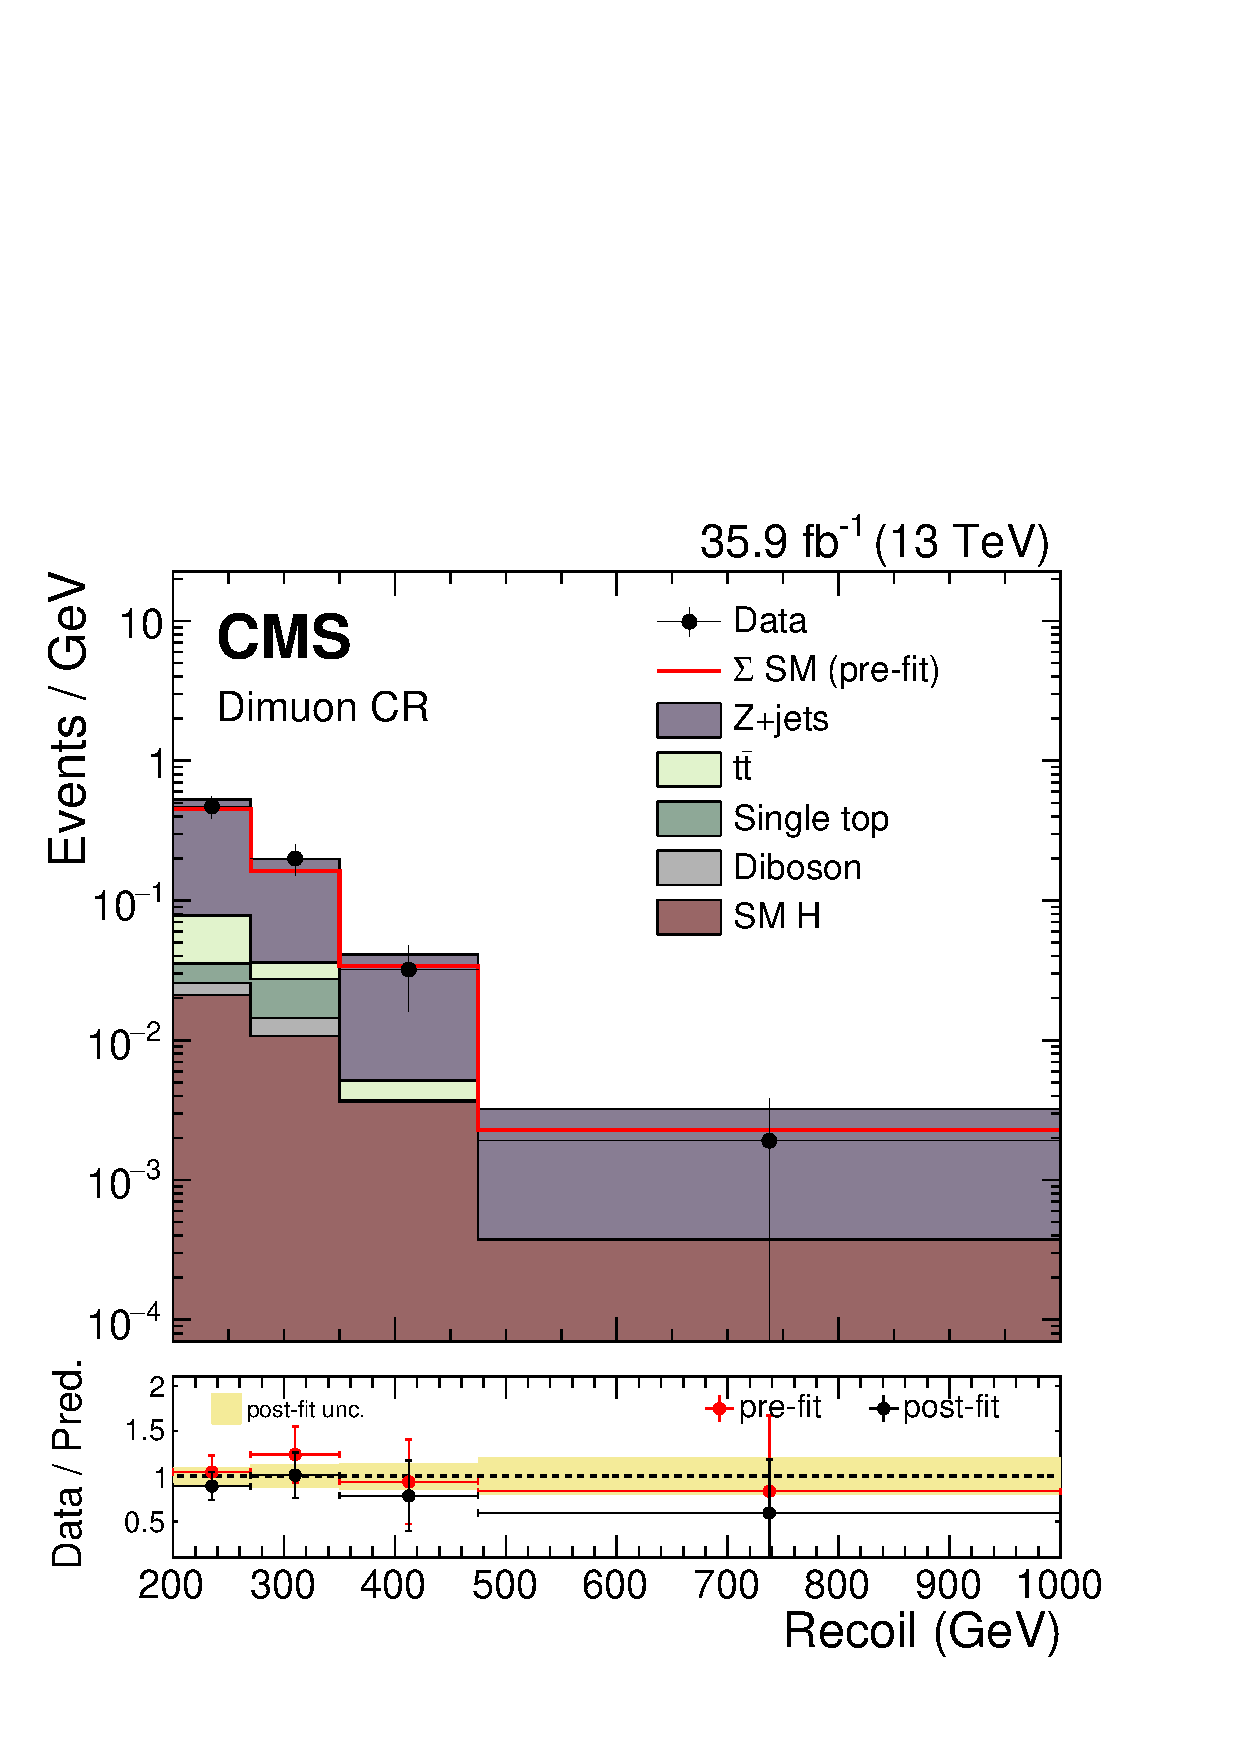
\includegraphics[width=0.4\textwidth]{figures/limits/MSDcorr_stackedPostfit_dimuon.pdf}}
 \subfloat{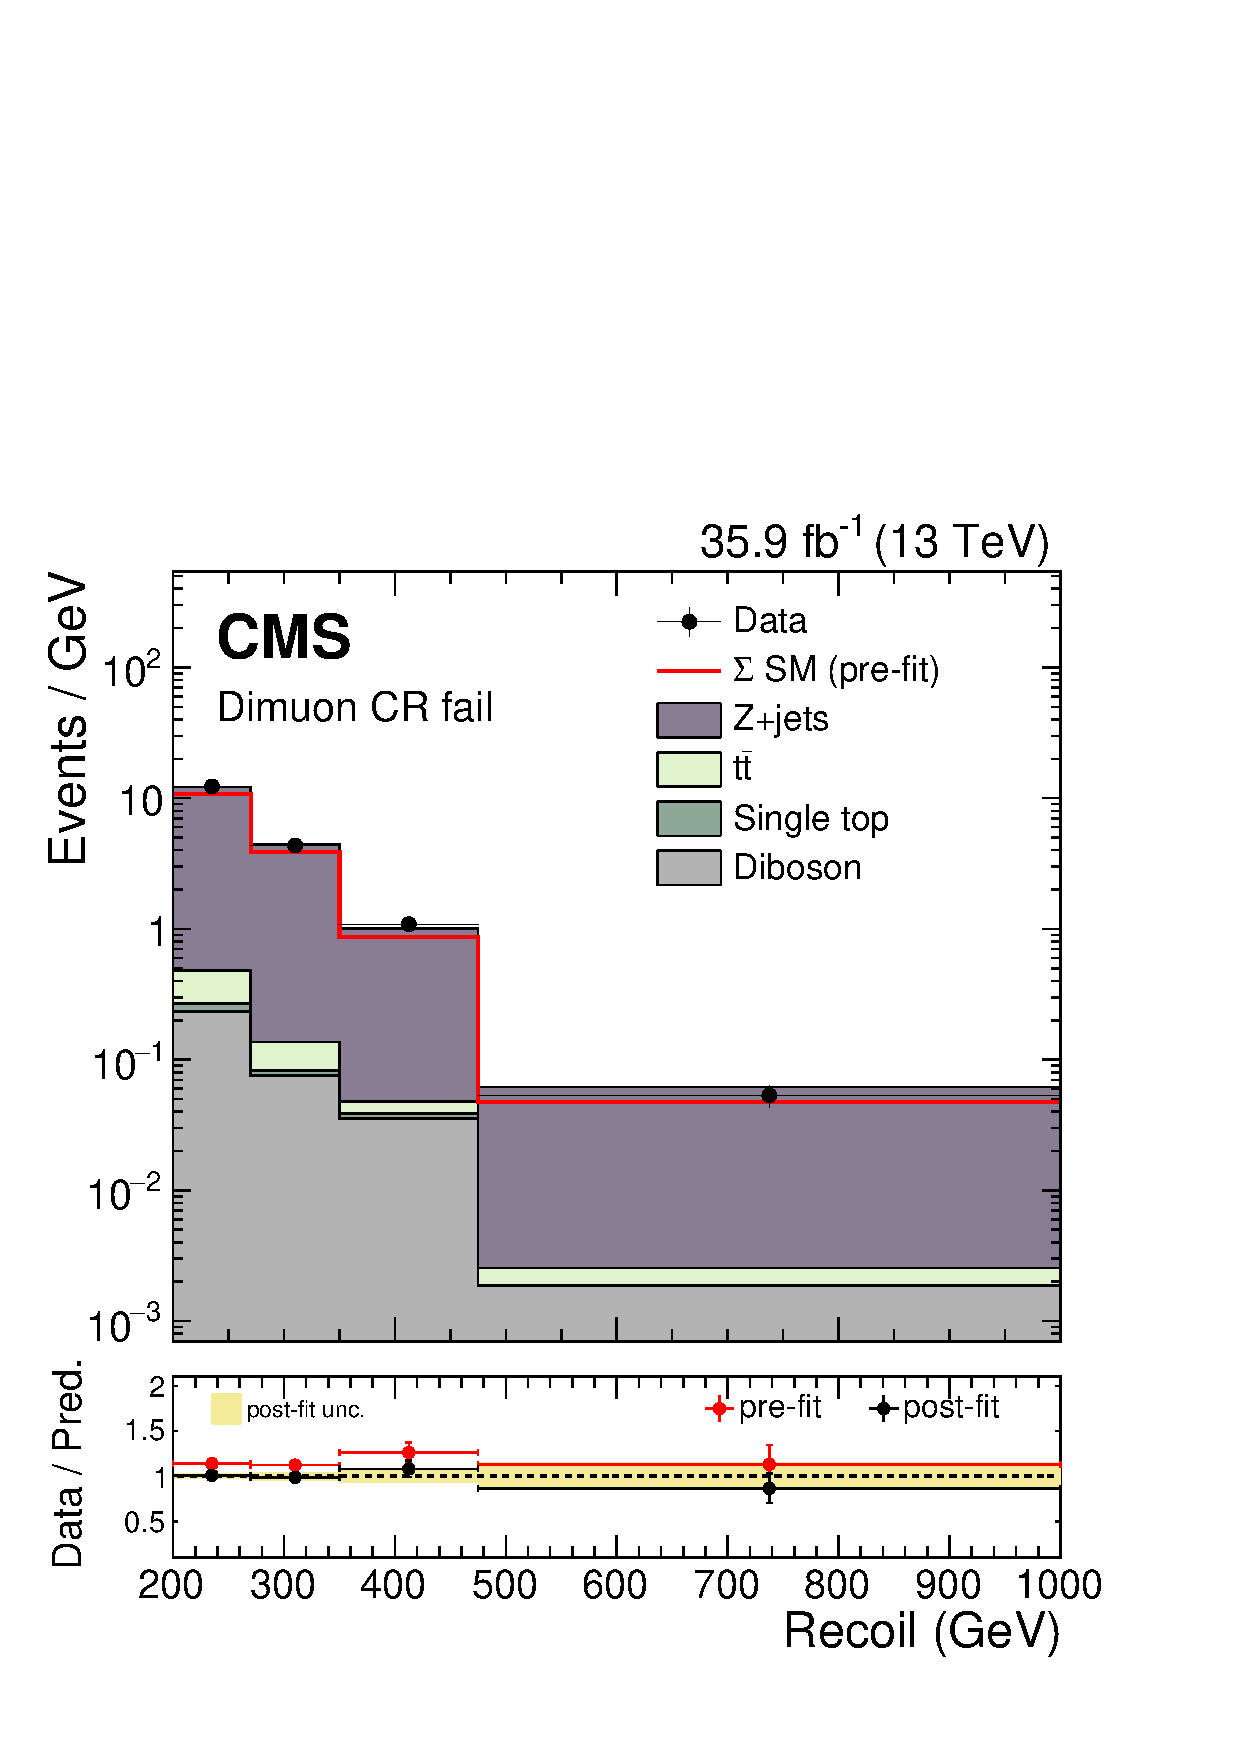
\includegraphics[width=0.4\textwidth]{figures/limits/MSDcorr_stackedPostfit_dimuon_fail.pdf}} \\
 \subfloat{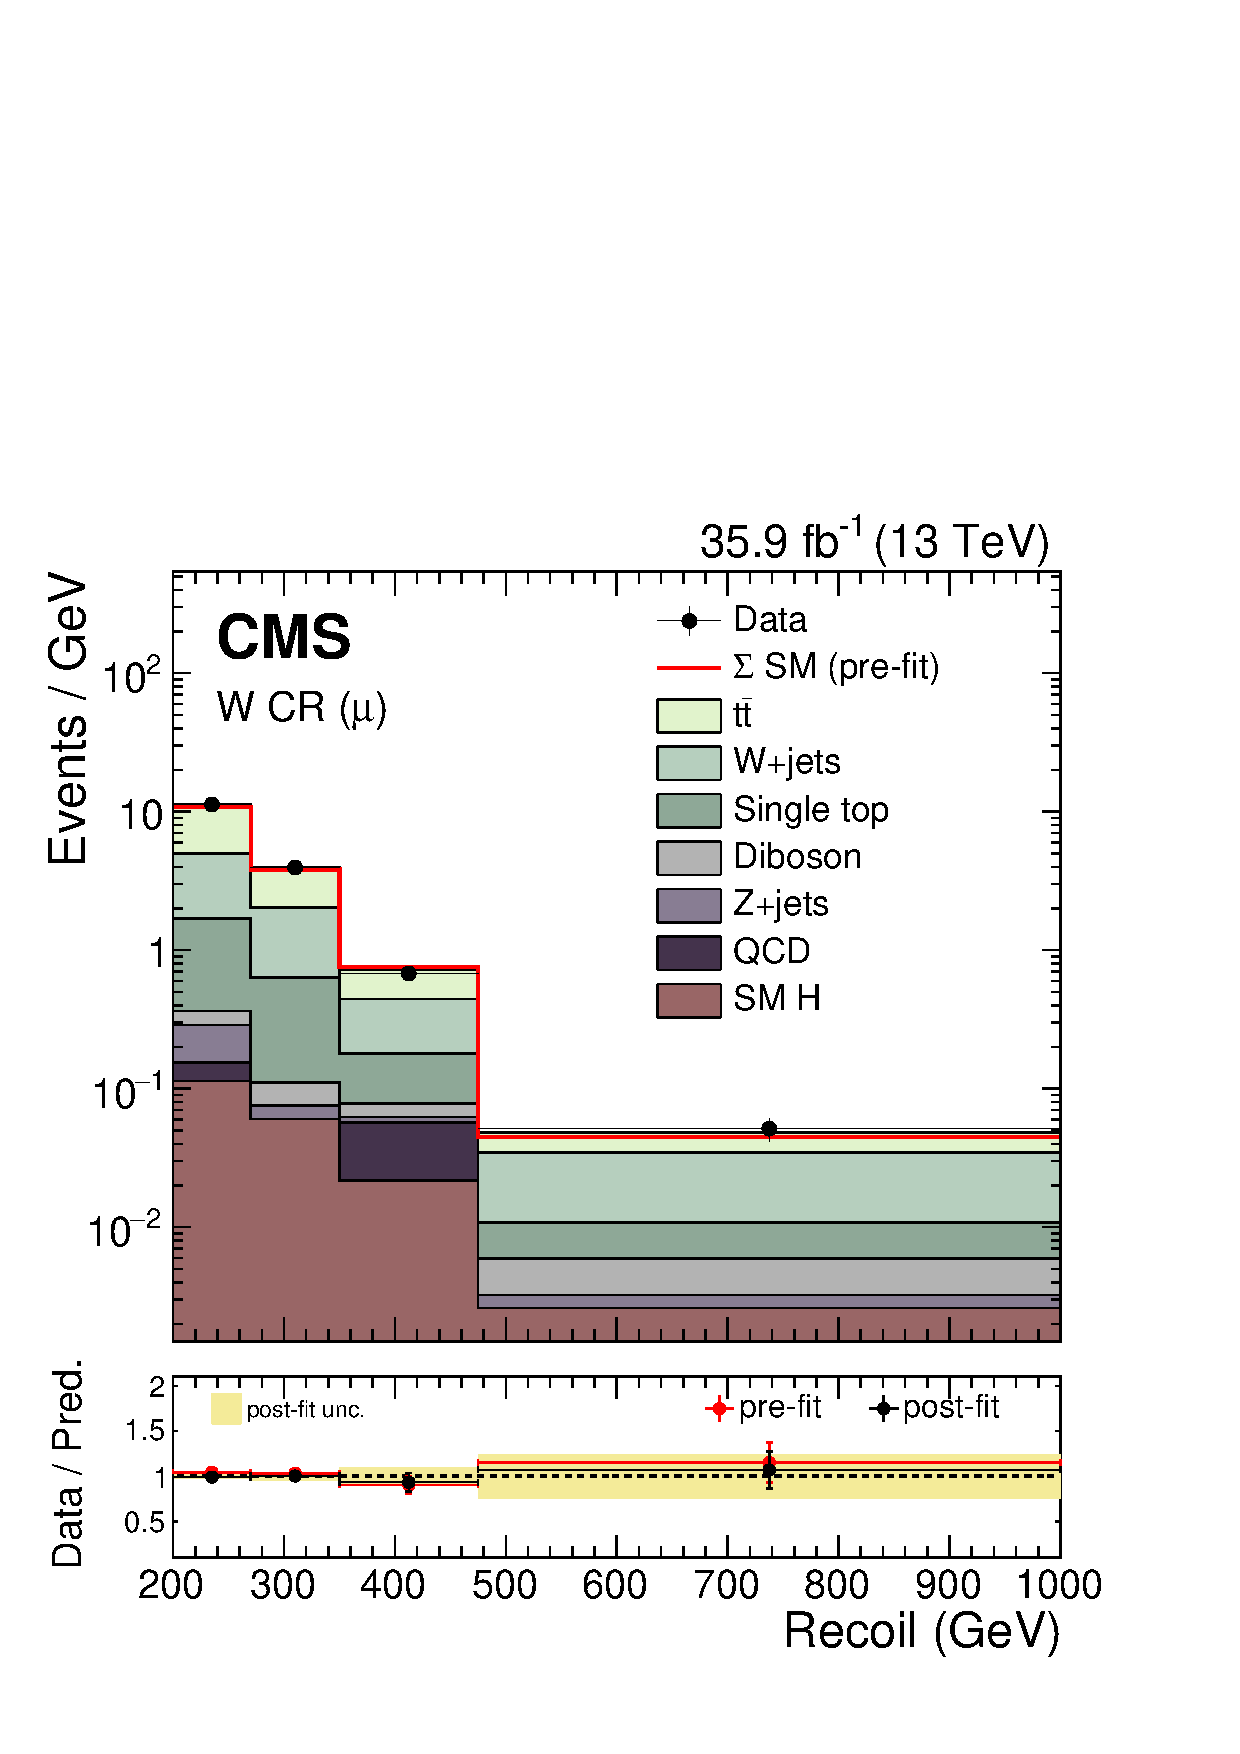
\includegraphics[width=0.4\textwidth]{figures/limits/MSDcorr_stackedPostfit_singlemuonw.pdf}}
 \subfloat{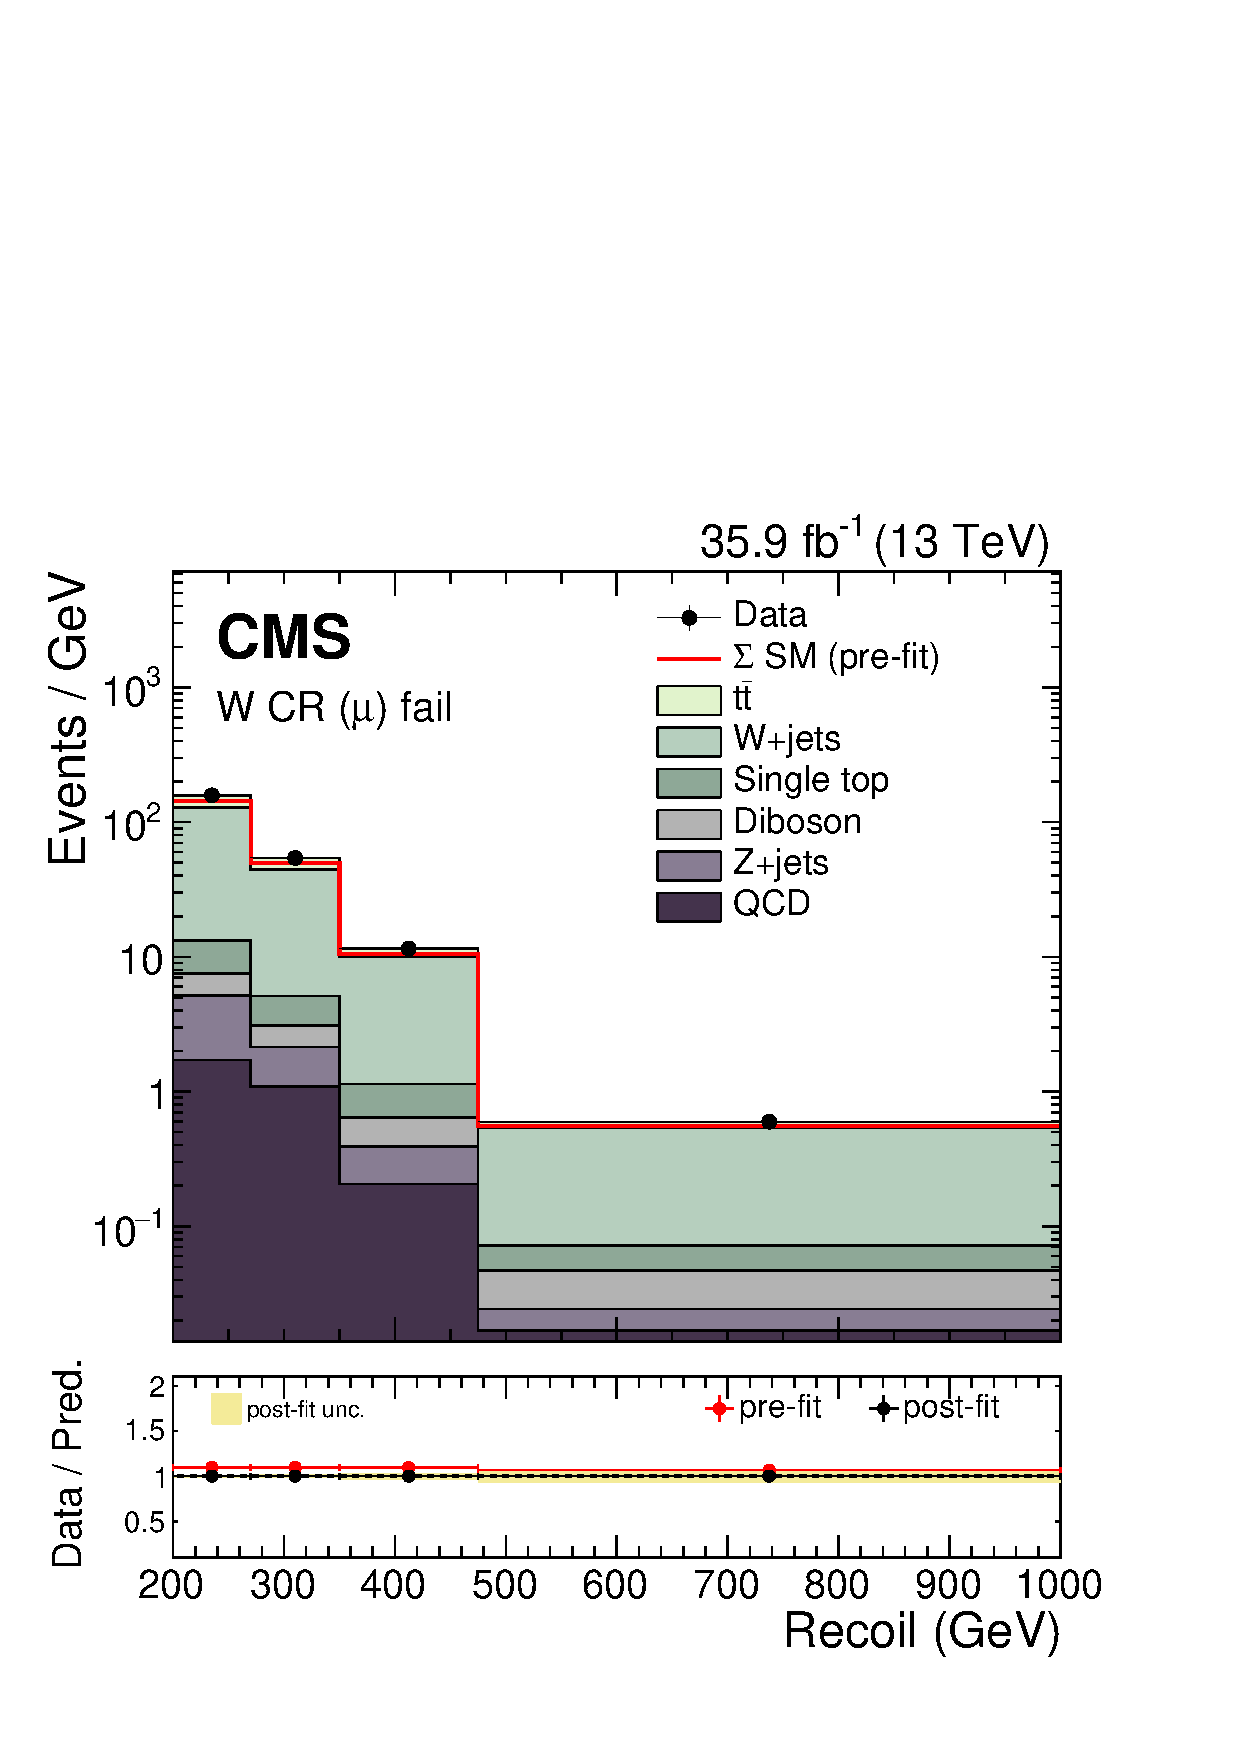
\includegraphics[width=0.4\textwidth]{figures/limits/MSDcorr_stackedPostfit_singlemuonw_fail.pdf}} \\
 \subfloat{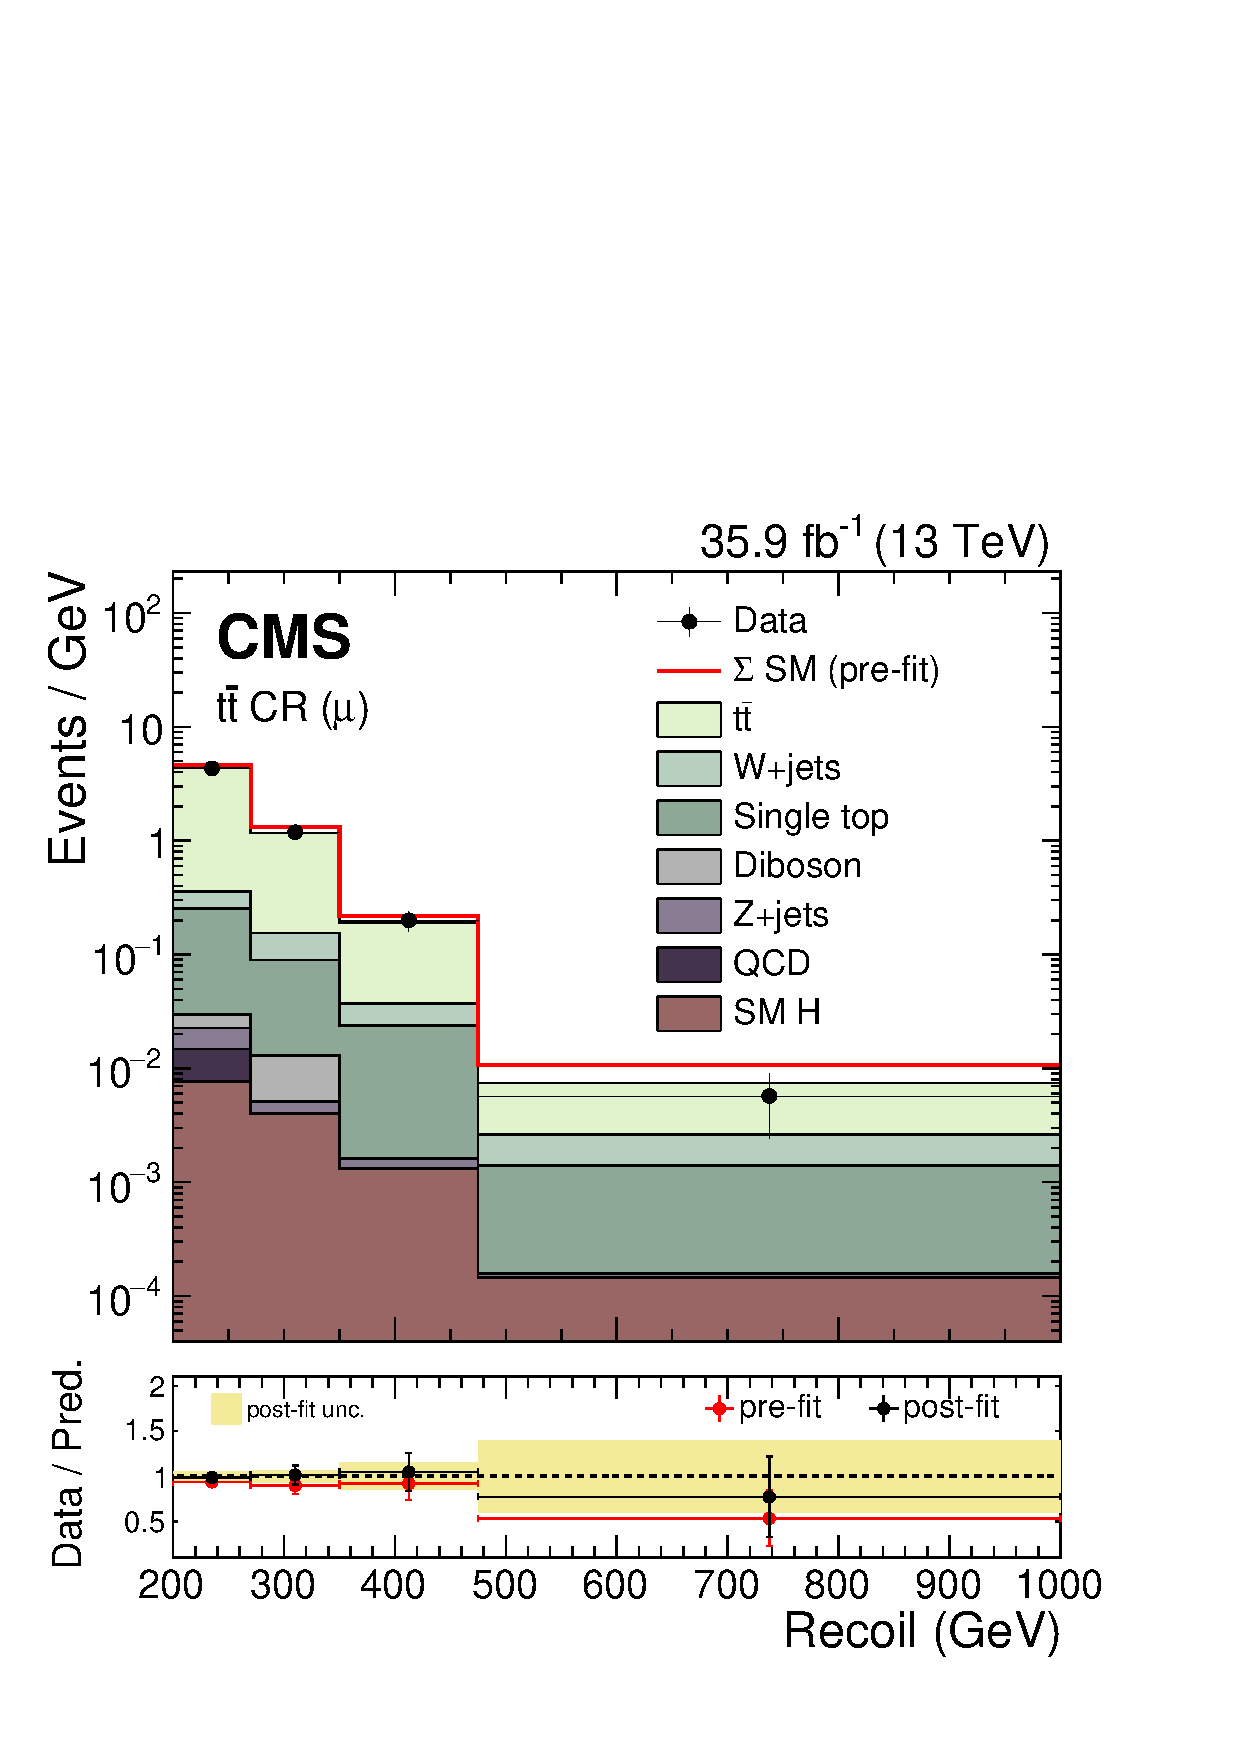
\includegraphics[width=0.4\textwidth]{figures/limits/MSDcorr_stackedPostfit_singlemuontop.pdf}} 
 \subfloat{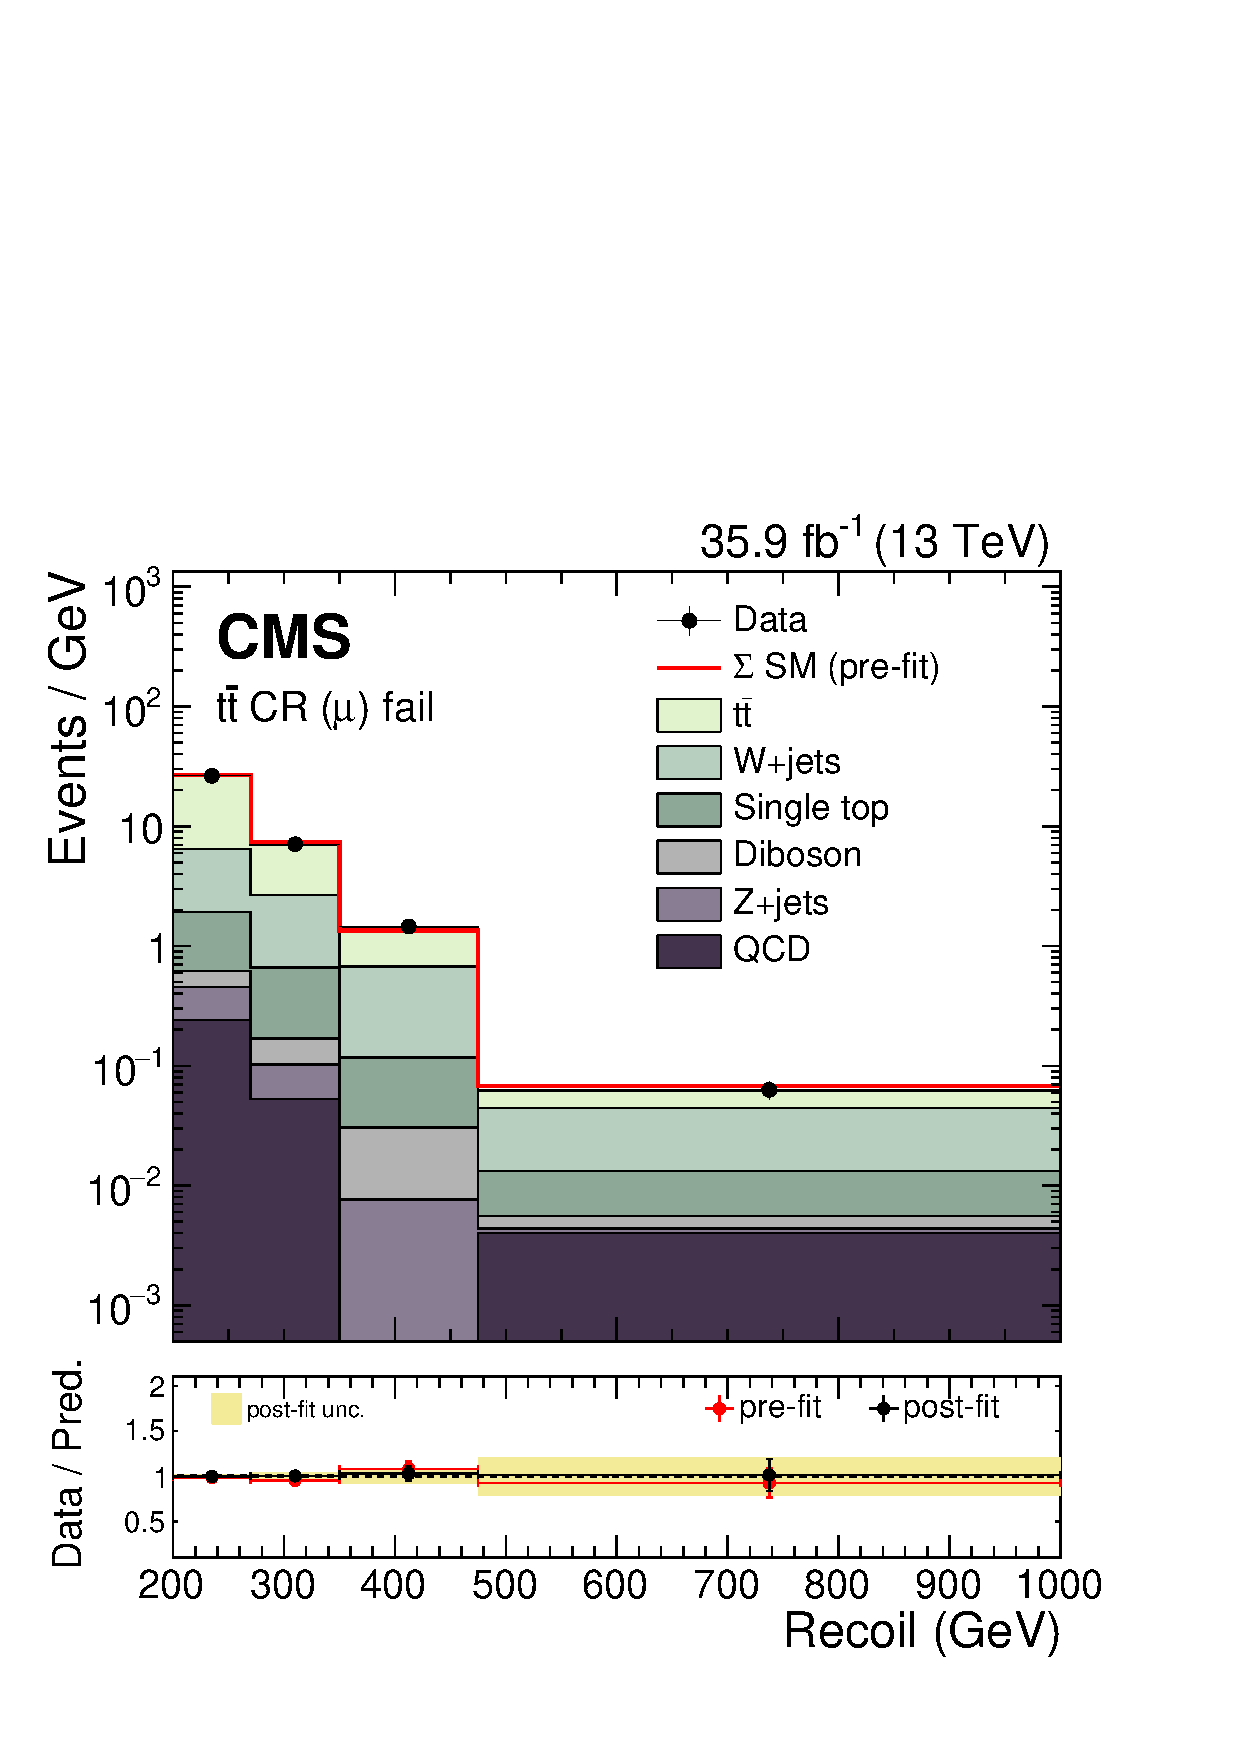
\includegraphics[width=0.4\textwidth]{figures/limits/MSDcorr_stackedPostfit_singlemuontop_fail.pdf}} \\
\caption{Postfit plots in the muon regions.}
\label{Fig_postfit_1}
\end{figure}

\begin{figure}
\centering
 \subfloat{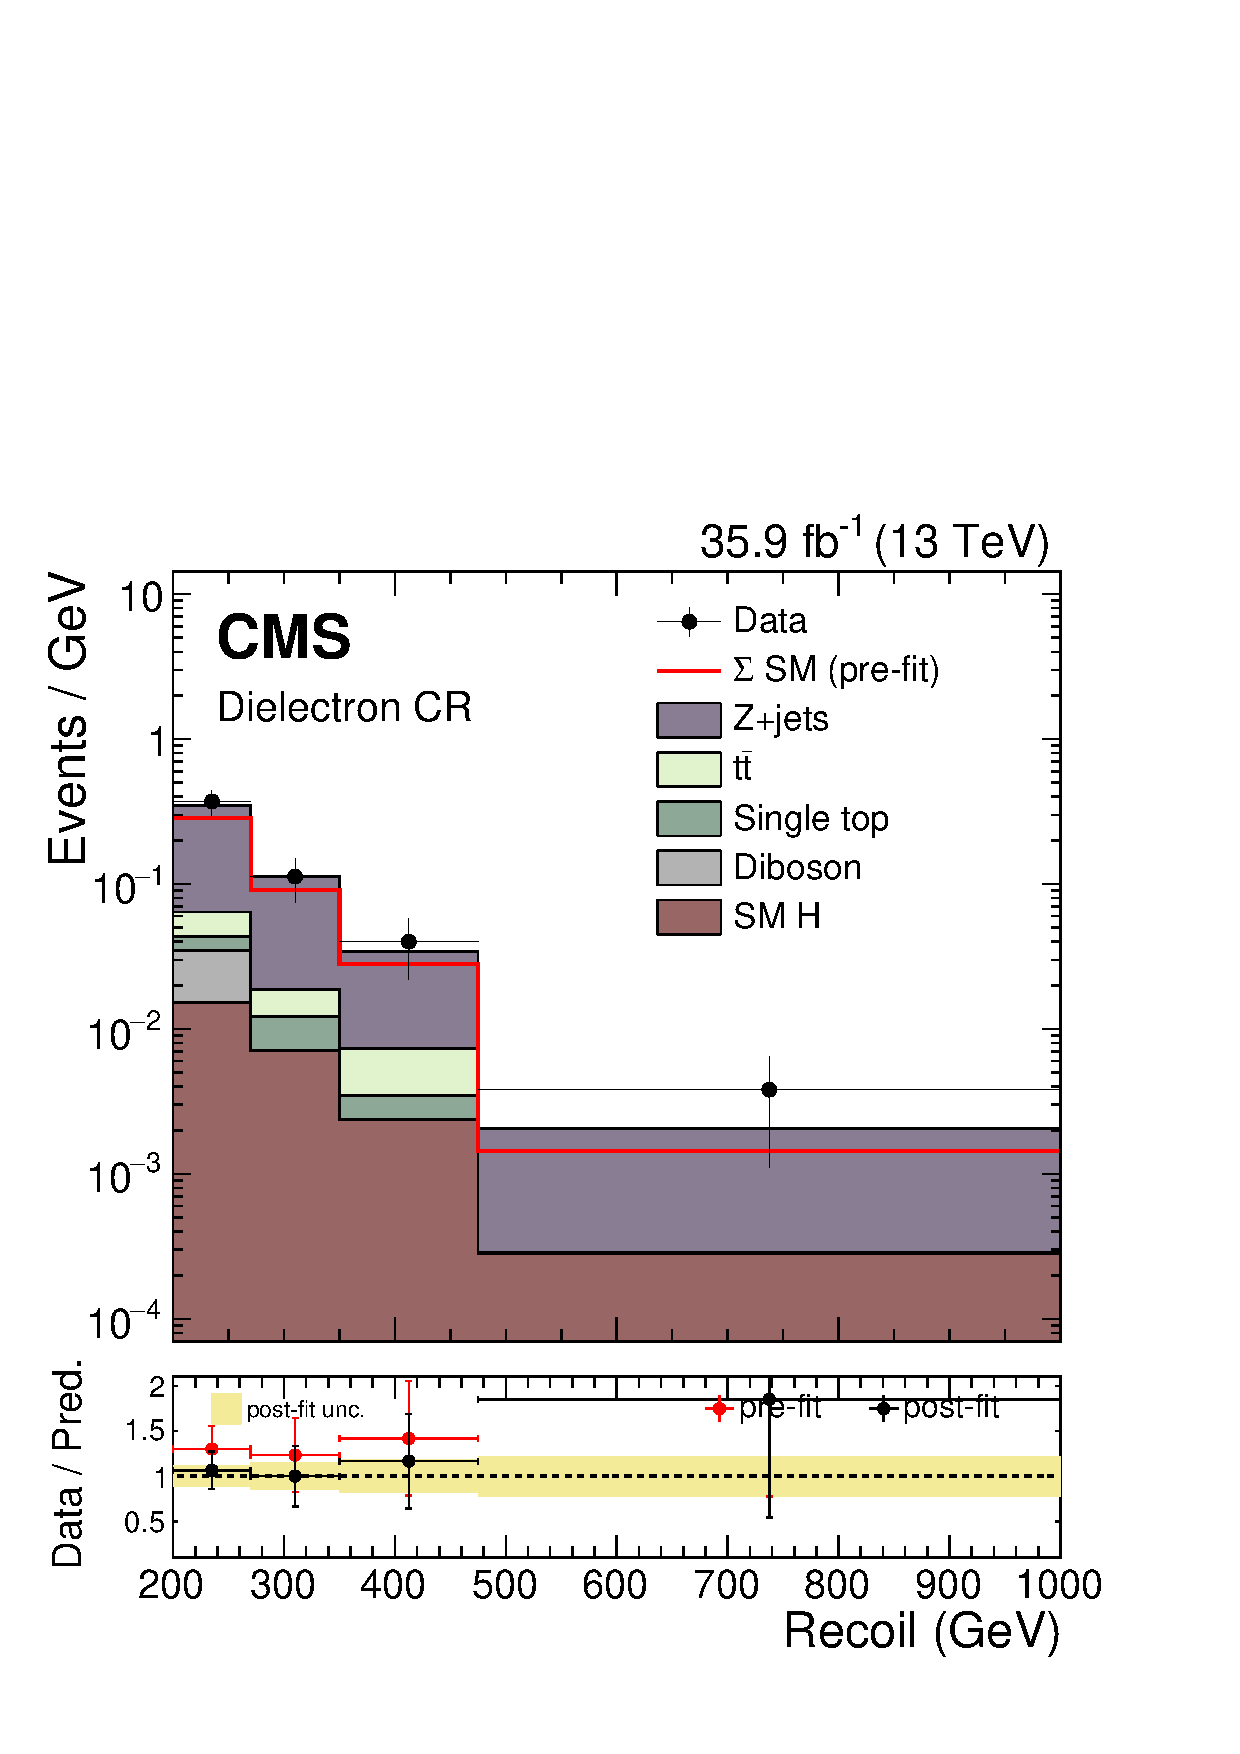
\includegraphics[width=0.4\textwidth]{figures/limits/MSDcorr_stackedPostfit_dielectron.pdf}}
 \subfloat{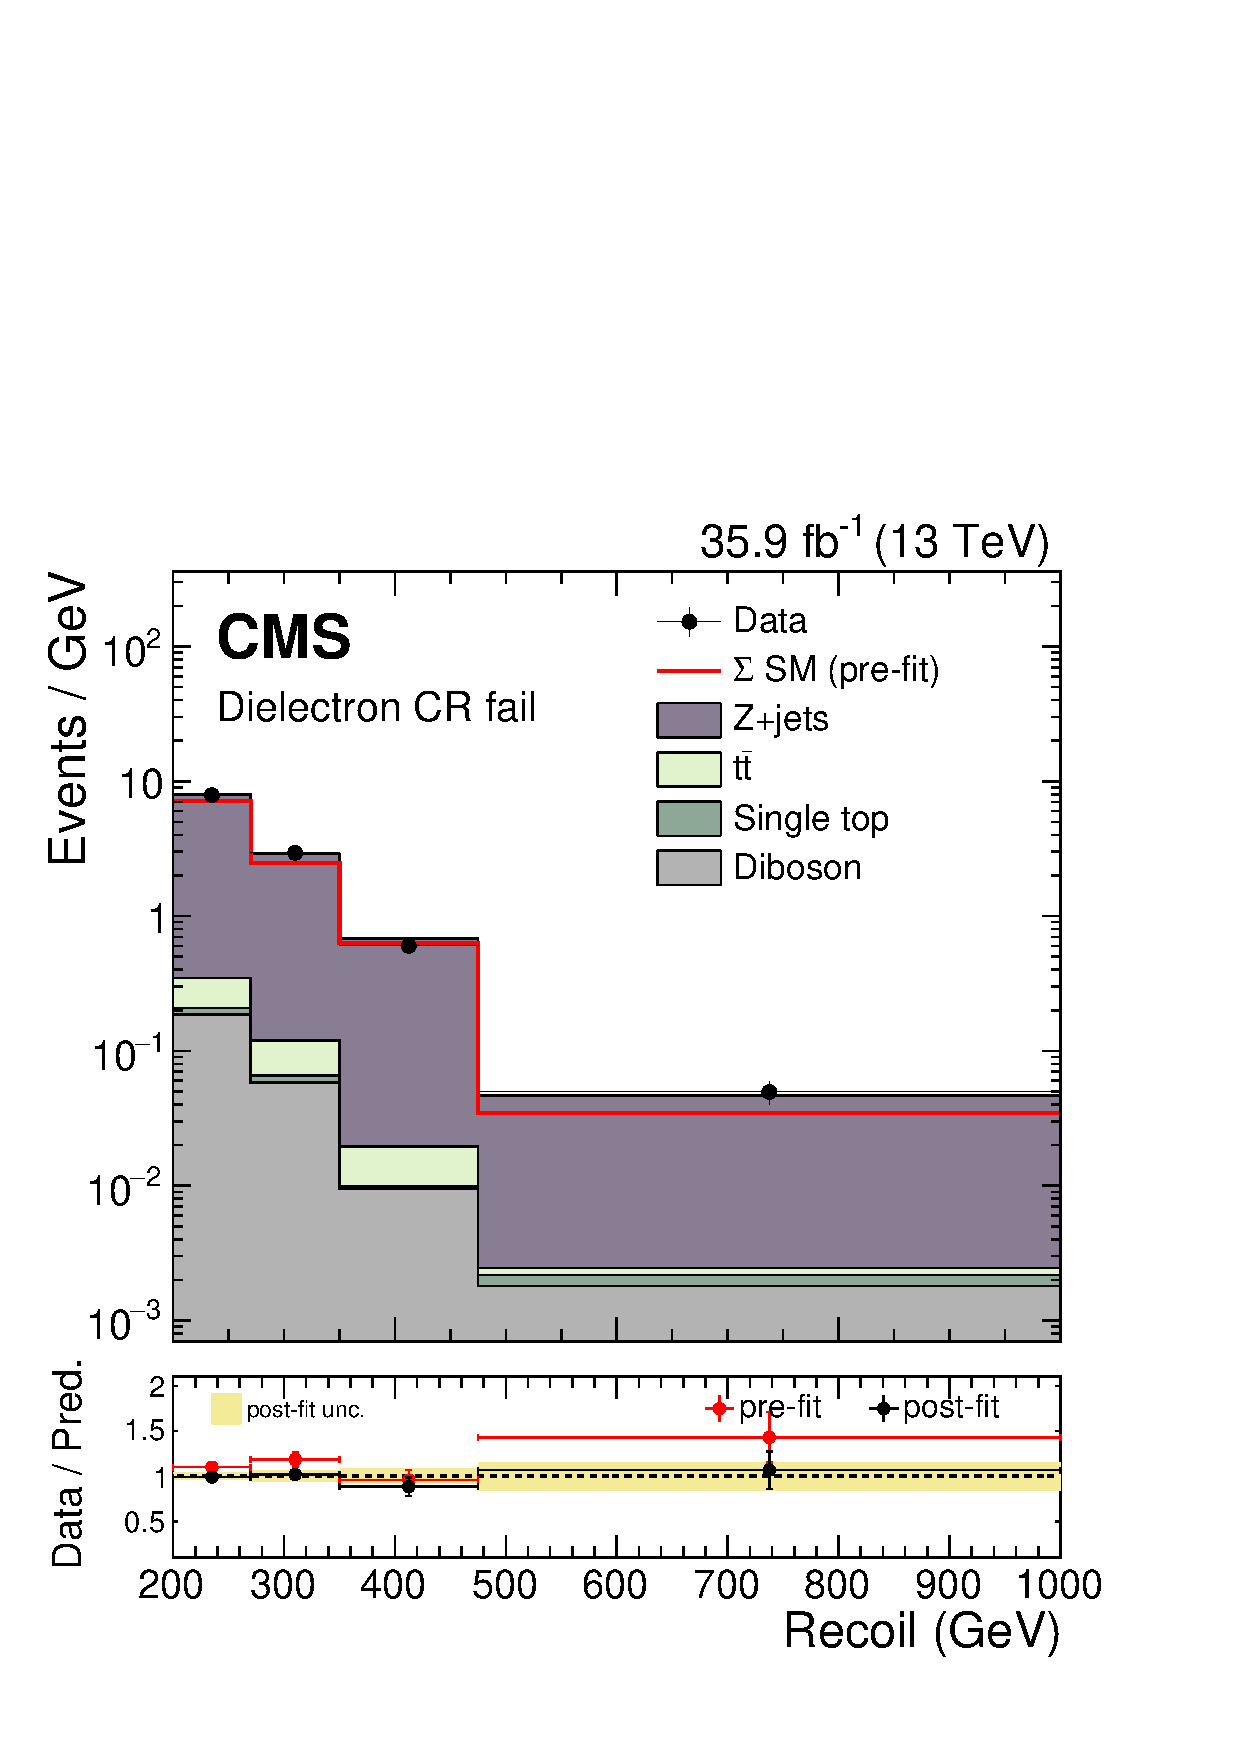
\includegraphics[width=0.4\textwidth]{figures/limits/MSDcorr_stackedPostfit_dielectron_fail.pdf}} \\
 \subfloat{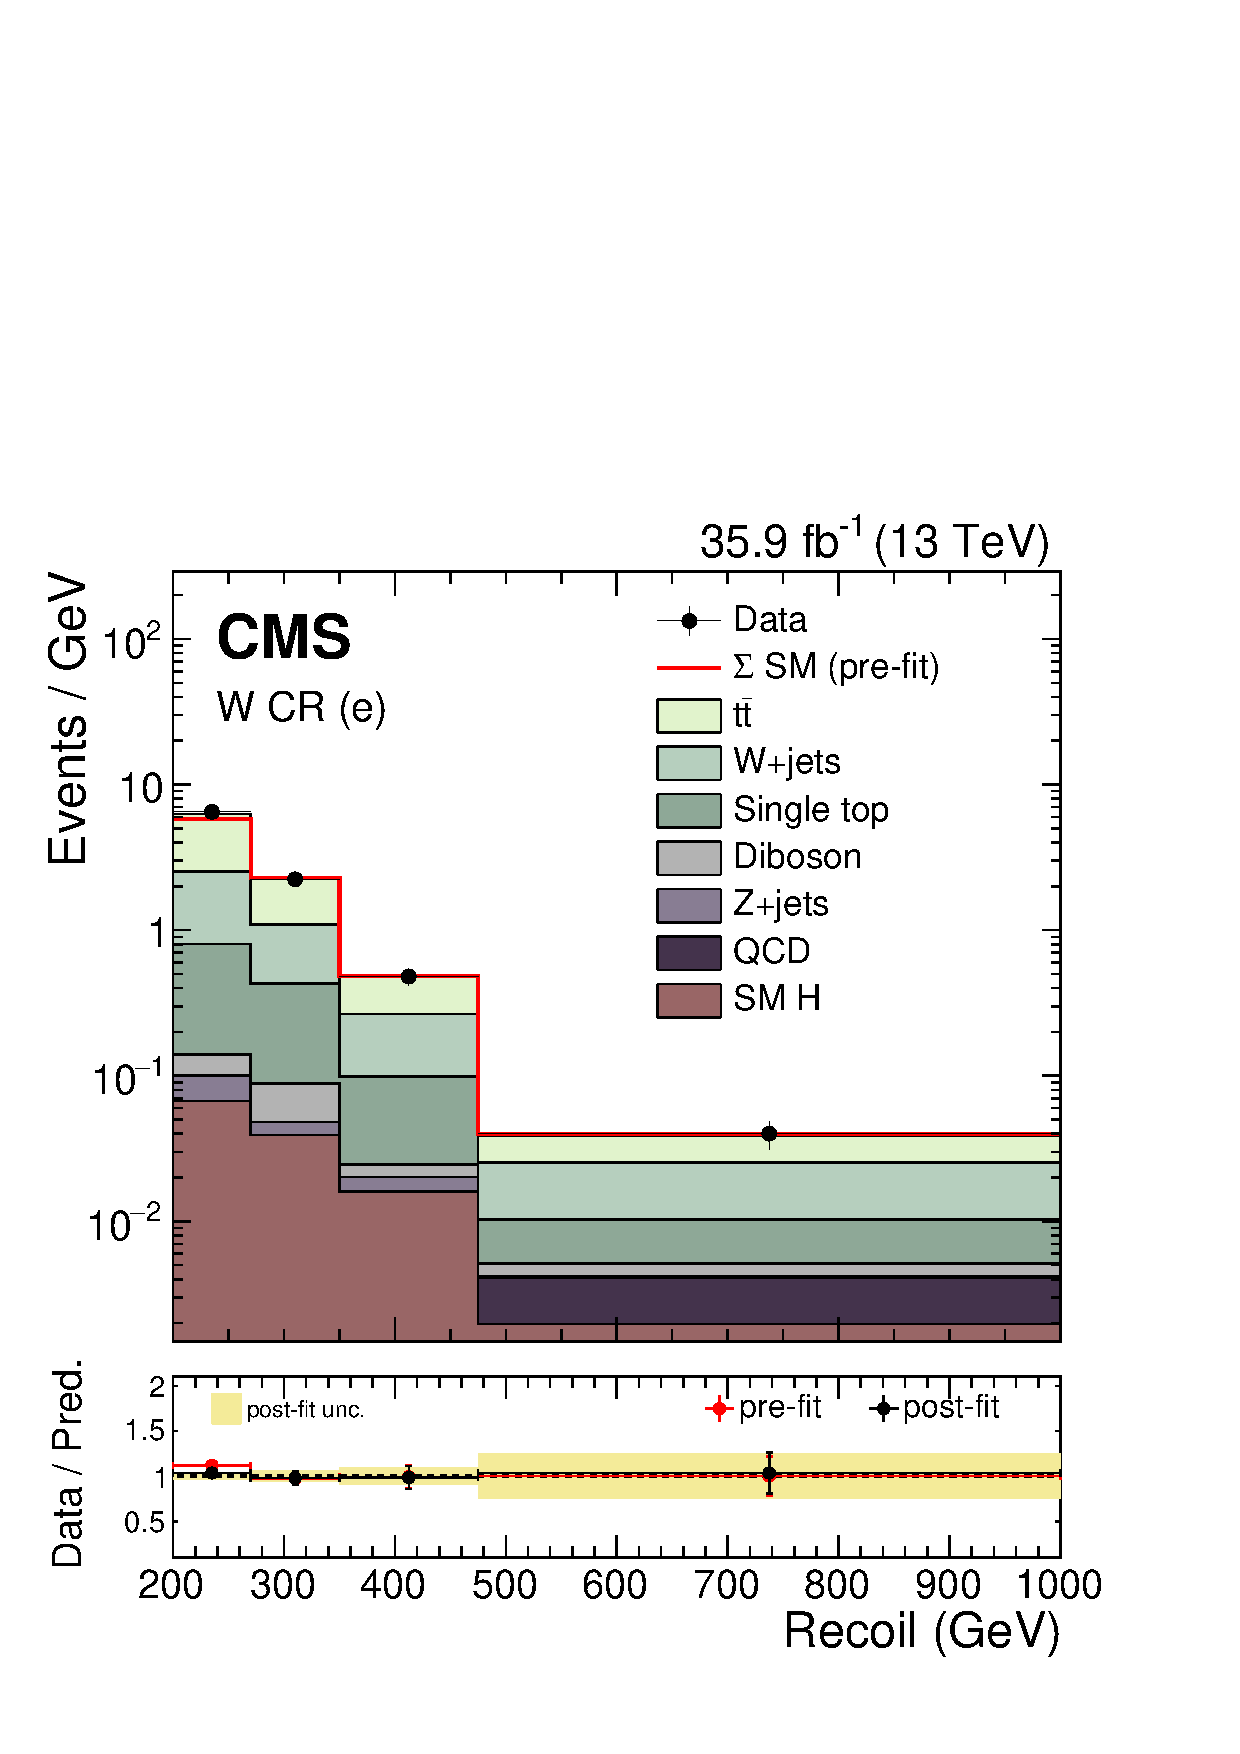
\includegraphics[width=0.4\textwidth]{figures/limits/MSDcorr_stackedPostfit_singleelectronw.pdf}}
 \subfloat{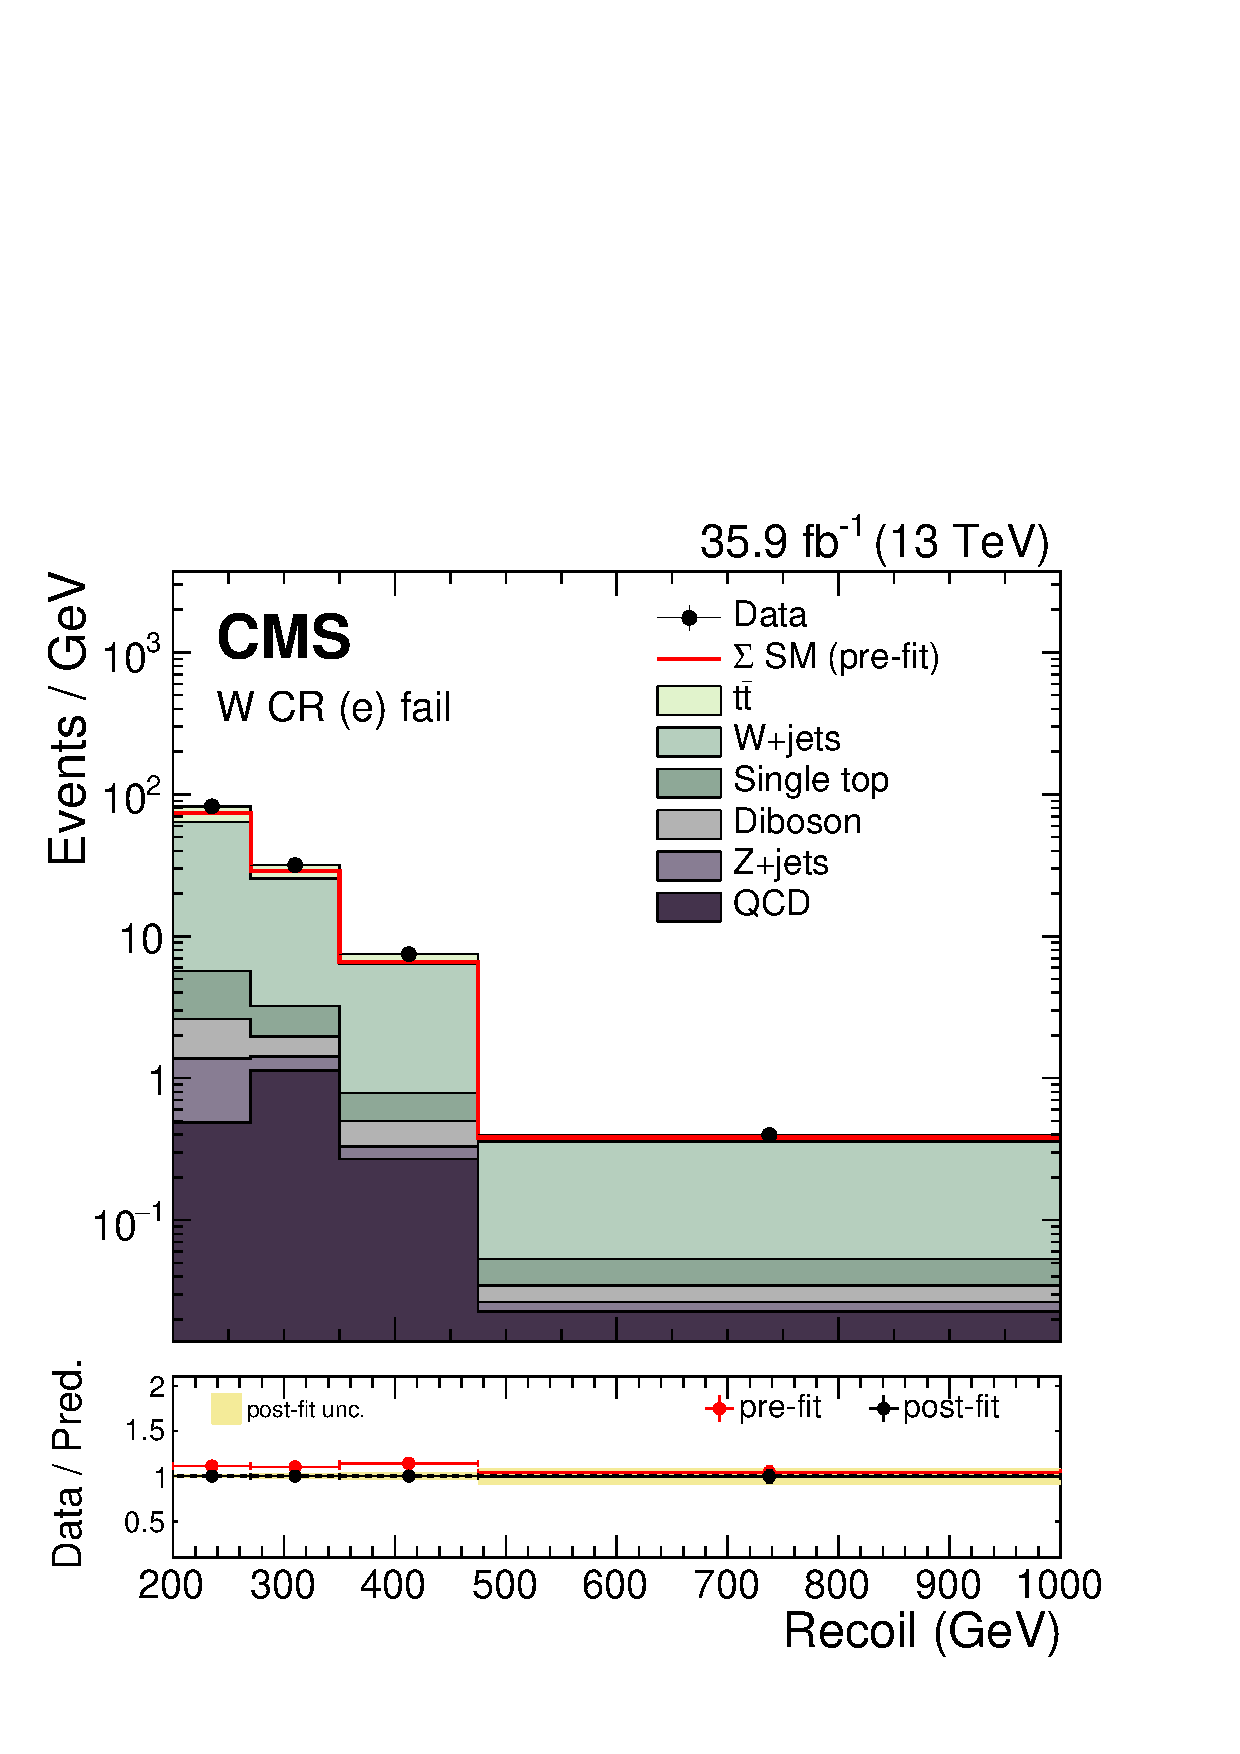
\includegraphics[width=0.4\textwidth]{figures/limits/MSDcorr_stackedPostfit_singleelectronw_fail.pdf}} \\
 \subfloat{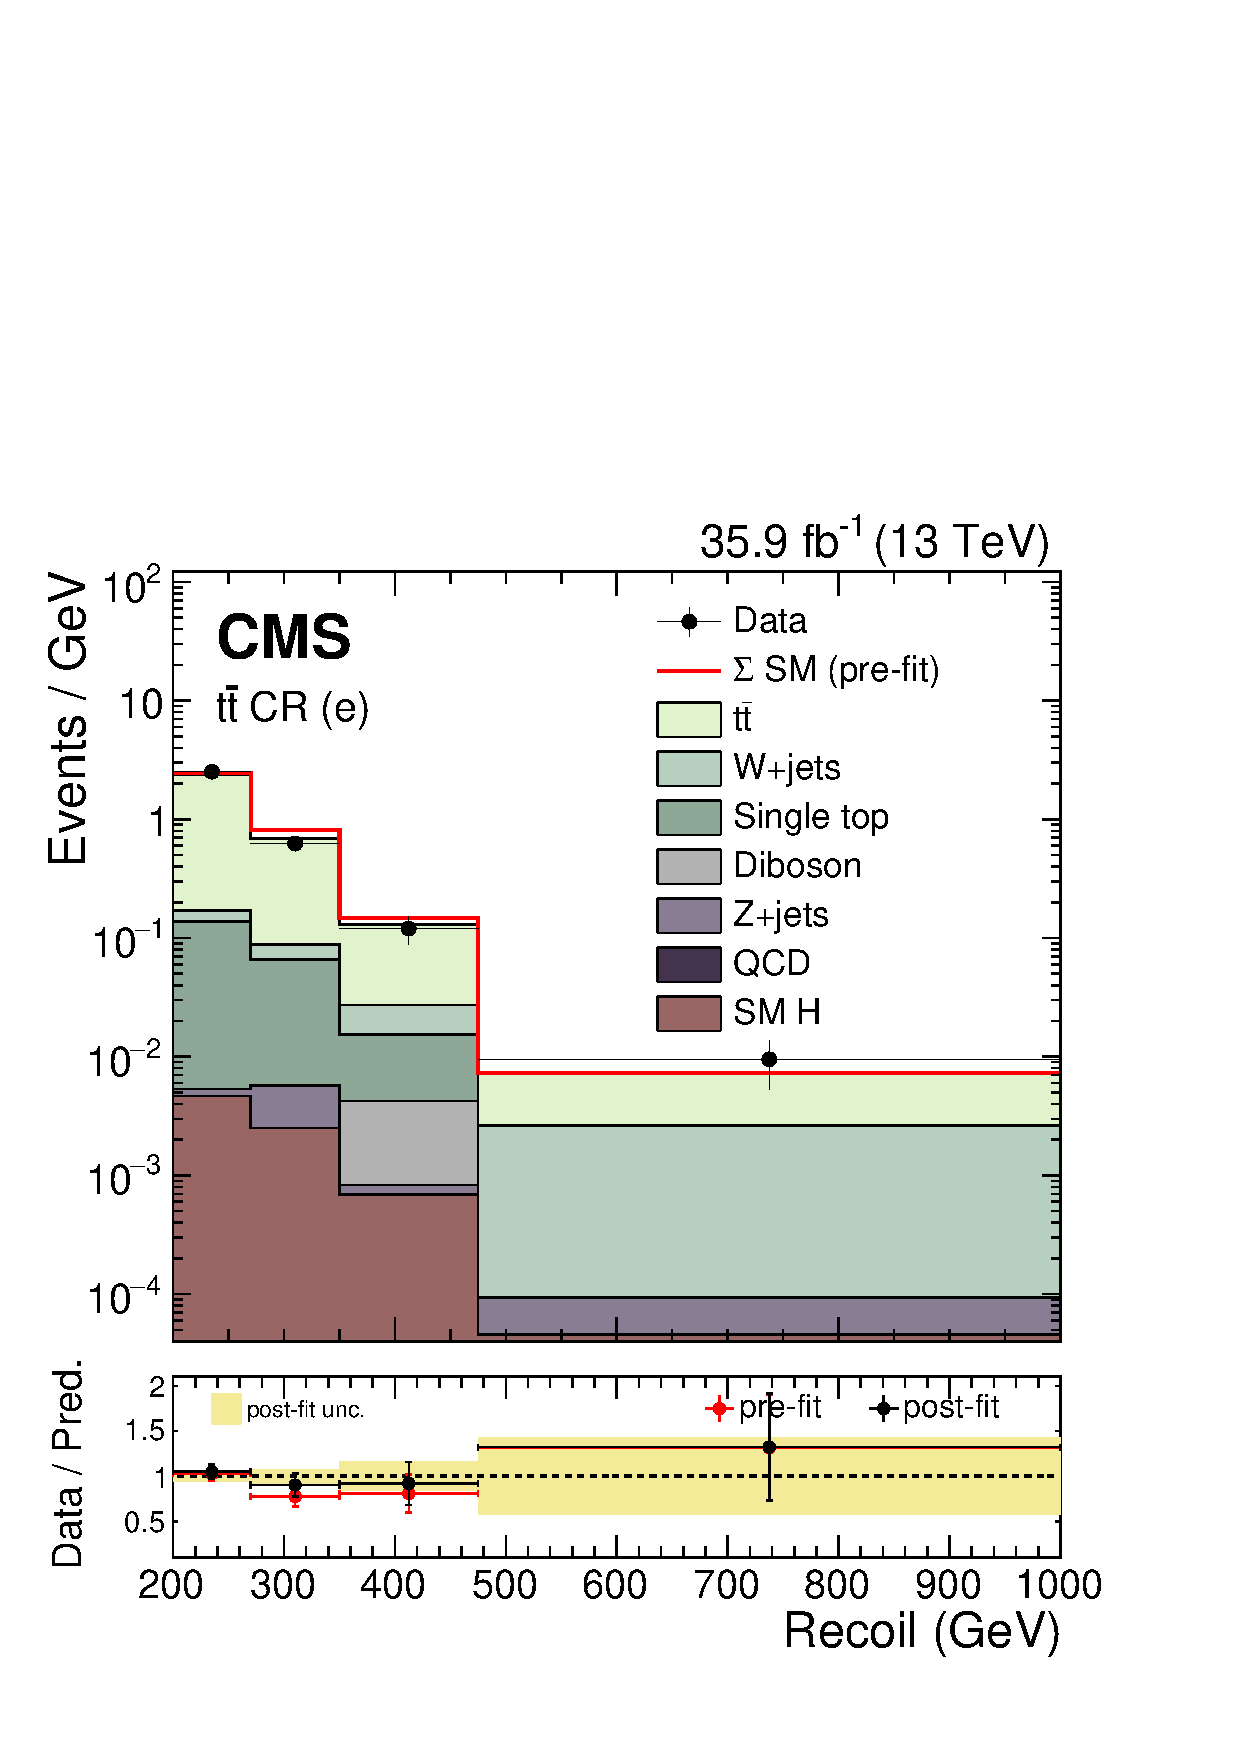
\includegraphics[width=0.4\textwidth]{figures/limits/MSDcorr_stackedPostfit_singleelectrontop.pdf}} 
 \subfloat{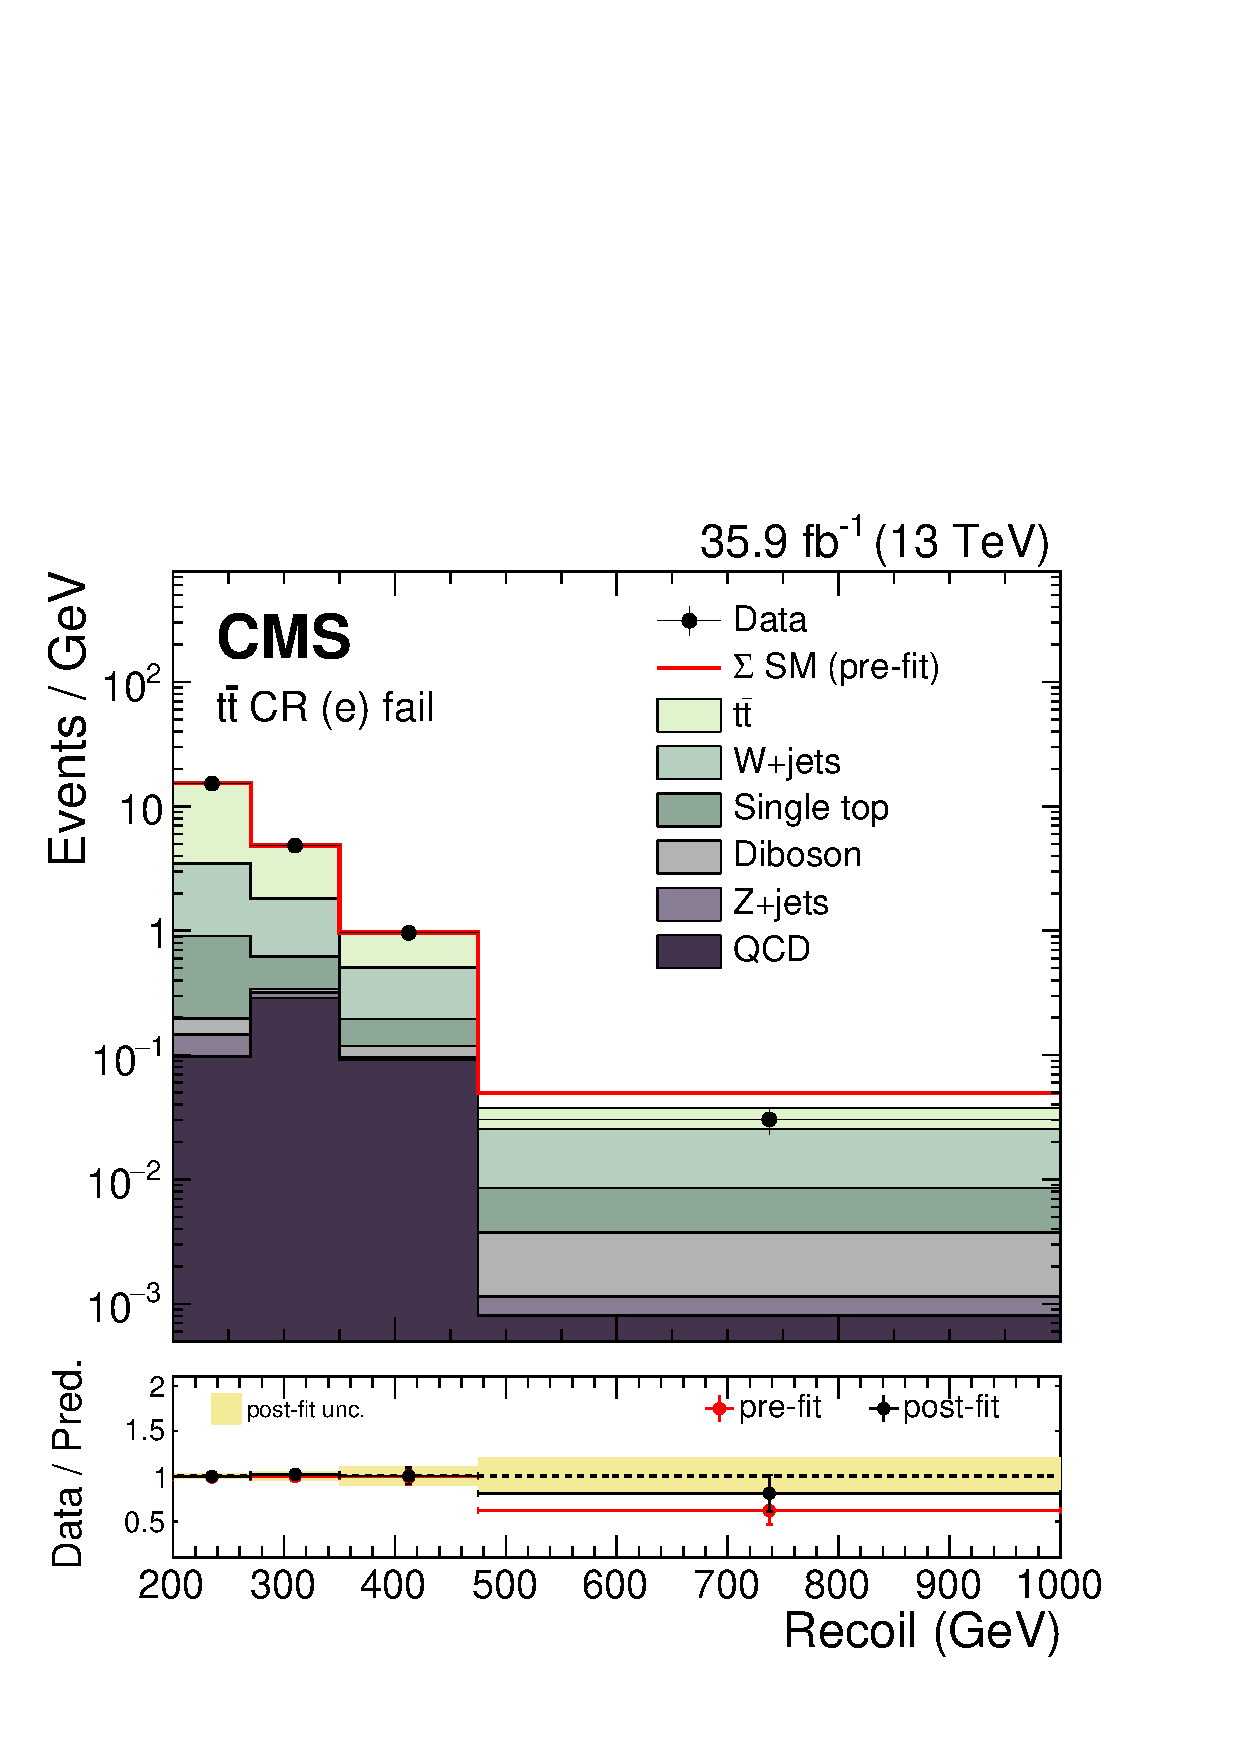
\includegraphics[width=0.4\textwidth]{figures/limits/MSDcorr_stackedPostfit_singleelectrontop_fail.pdf}} \\
\caption{Postfit plots in the electron regions.}
\label{Fig_postfit_2}
\end{figure}

\begin{figure}
\centering
 \subfloat{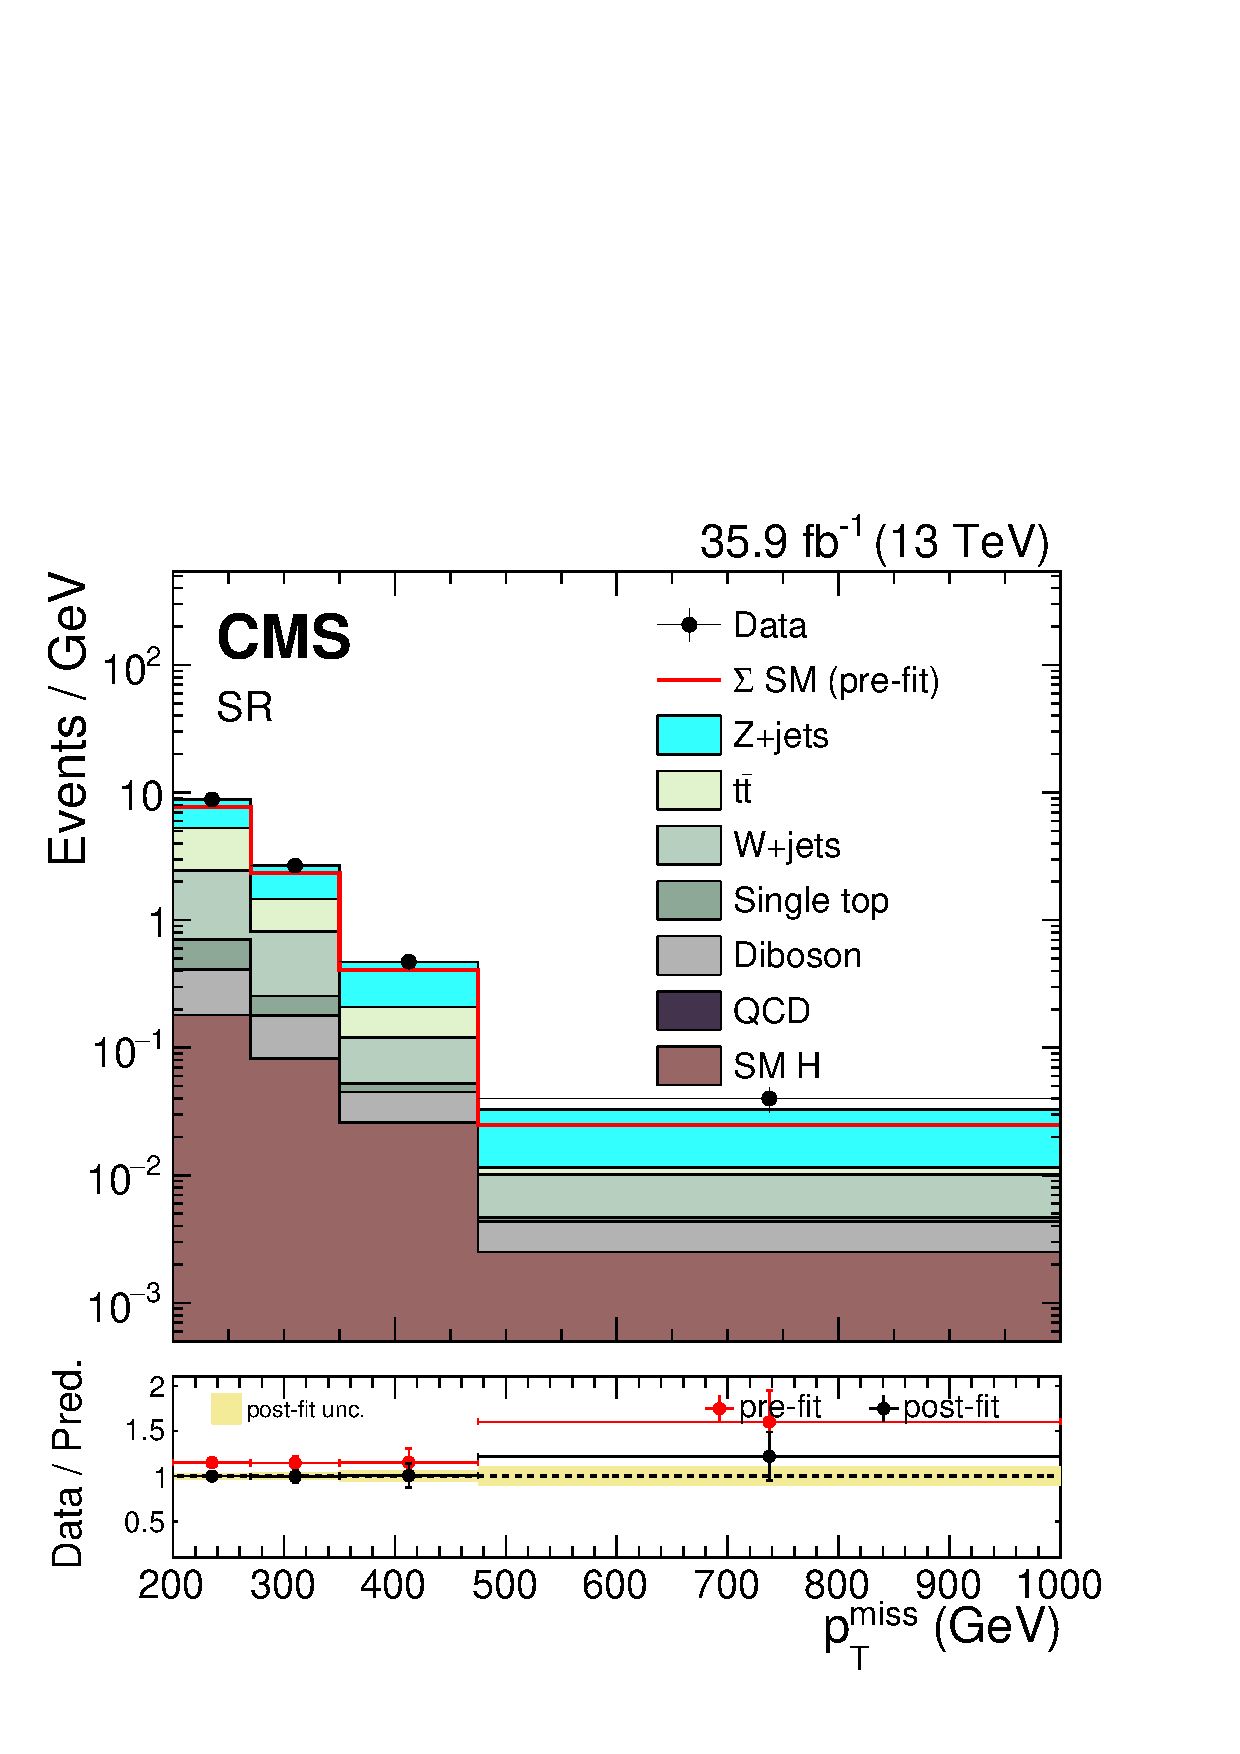
\includegraphics[width=0.4\textwidth]{figures/limits/MSDcorr_stackedPostfit_signal.pdf}}
 \subfloat{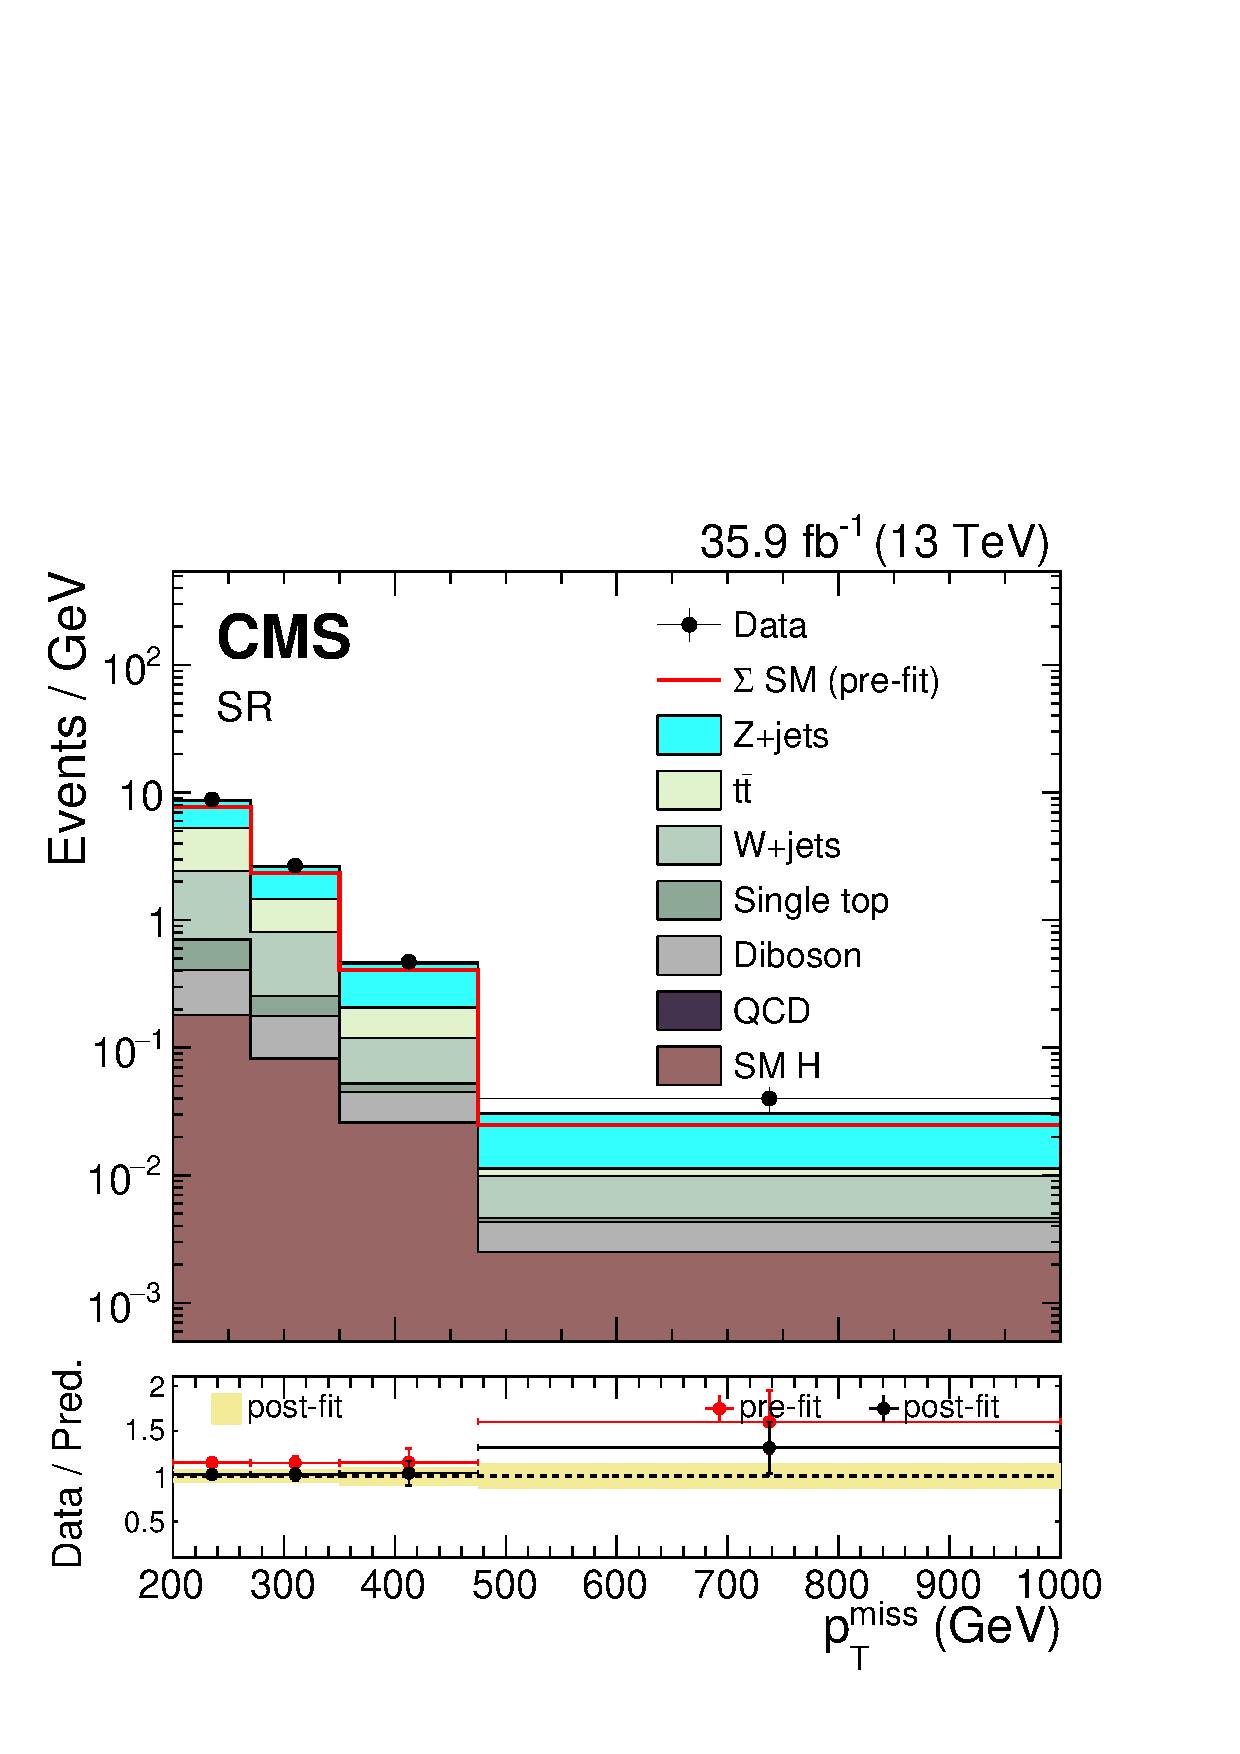
\includegraphics[width=0.4\textwidth]{figures/limits/MSDcorr_stackedPostfit_signal_masked.pdf}} \\
\caption{Left: postfit background expectations in the signal region evaluated after performing a combined fit to the data in all the control regions and the signal region. Right: postfit background expectations in the signal region evaluated after performing a combined fit to the data in all the control regions, but excluding the signal region.}
\label{Fig_postfit_3}
\end{figure}

The mass sideband of the signal region ($50<m_{\text{SD}}<100$\,GeV and $150<m_{\text{SD}}<200$\,GeV) is not part of the fit, but is used to perform a validation of the scale factors that the main backgrounds receive in the fit (e.g. the ratio of post- and pre-fit yields for DY as determined in the very pure dilepton CRs in the four recoil bins). Fig.~\ref{Fig_sideband} shows the prefit \ptmiss distribution in the sideband as well as the same distribution with the scale factors obtained in the fit applied to the V+jets and \ttbar~backgrounds. 

\begin{figure}
\centering
 \subfloat{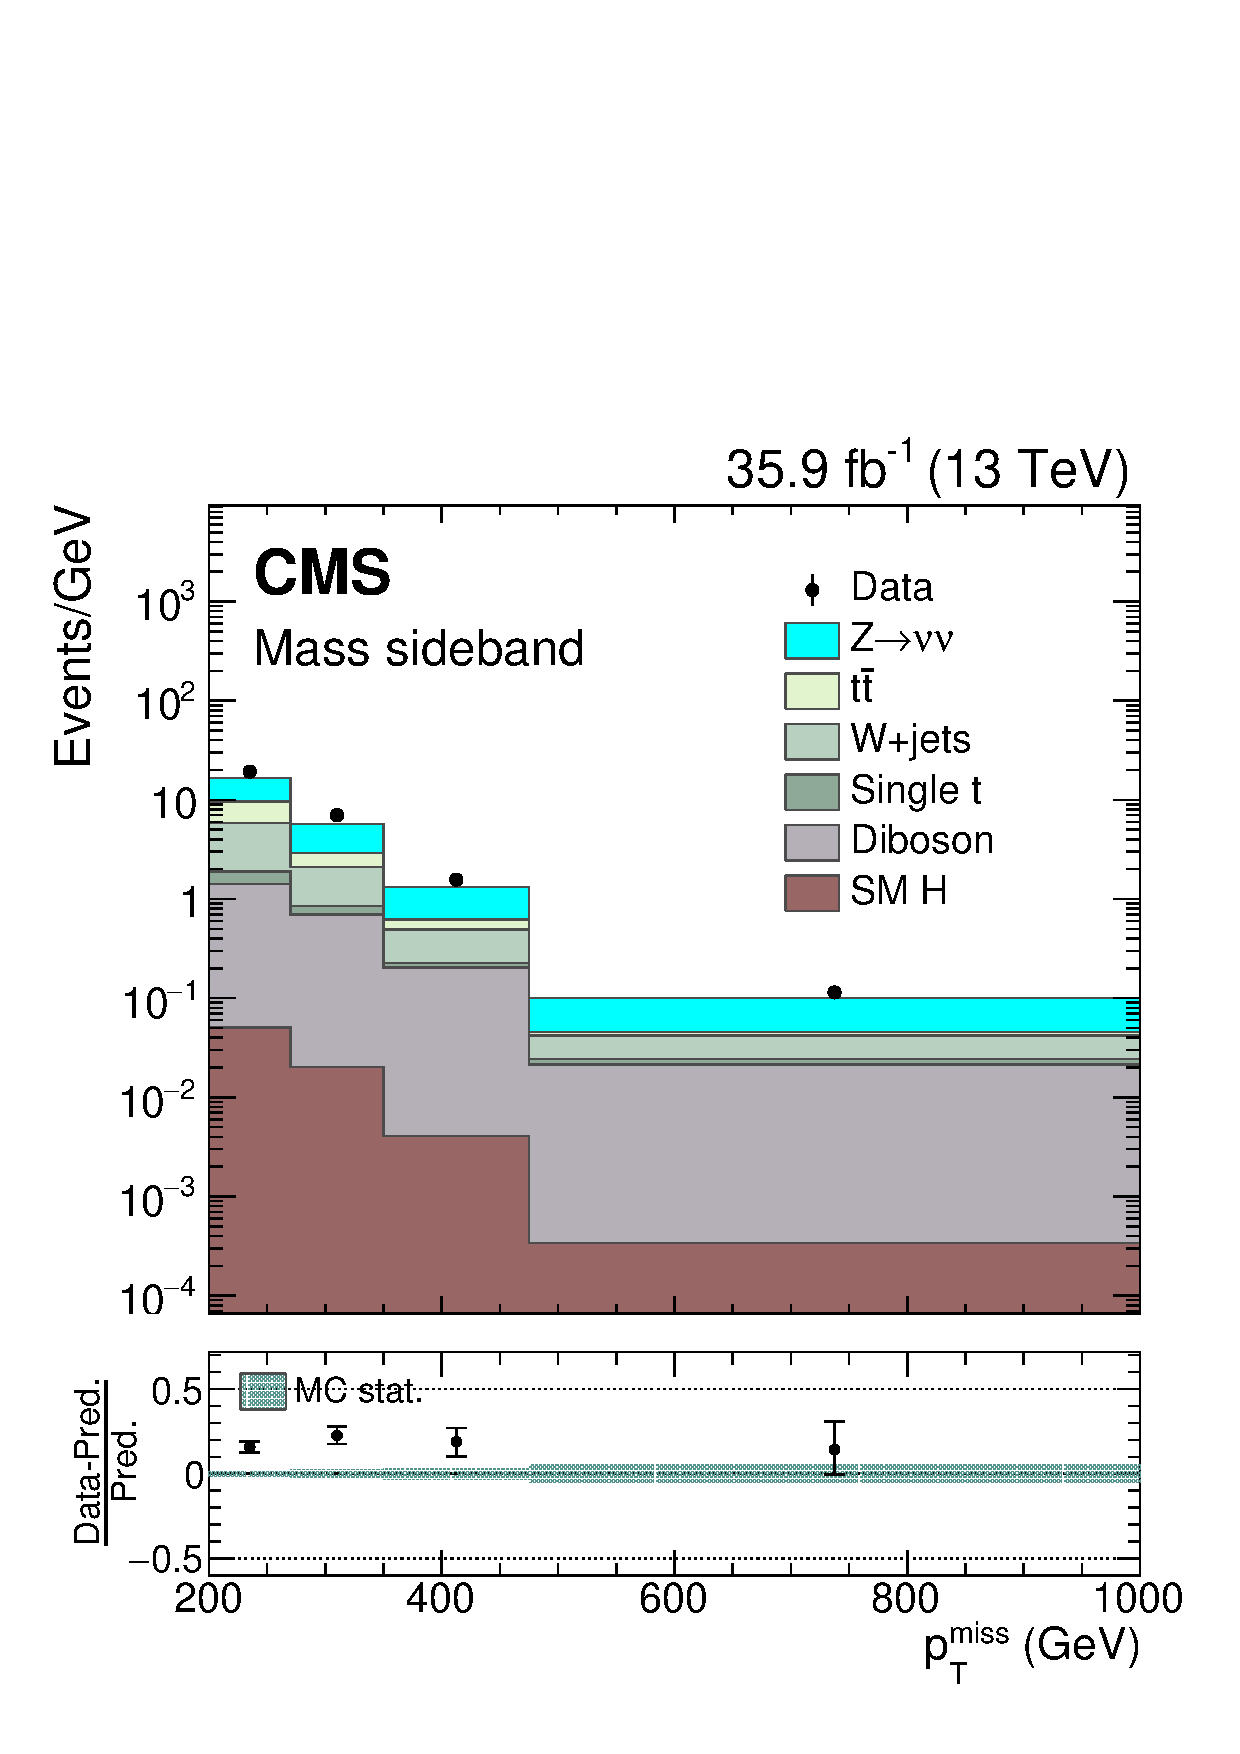
\includegraphics[width=0.4\textwidth]{figures/dataMC/cr_znunu_MET2.pdf}}
 \subfloat{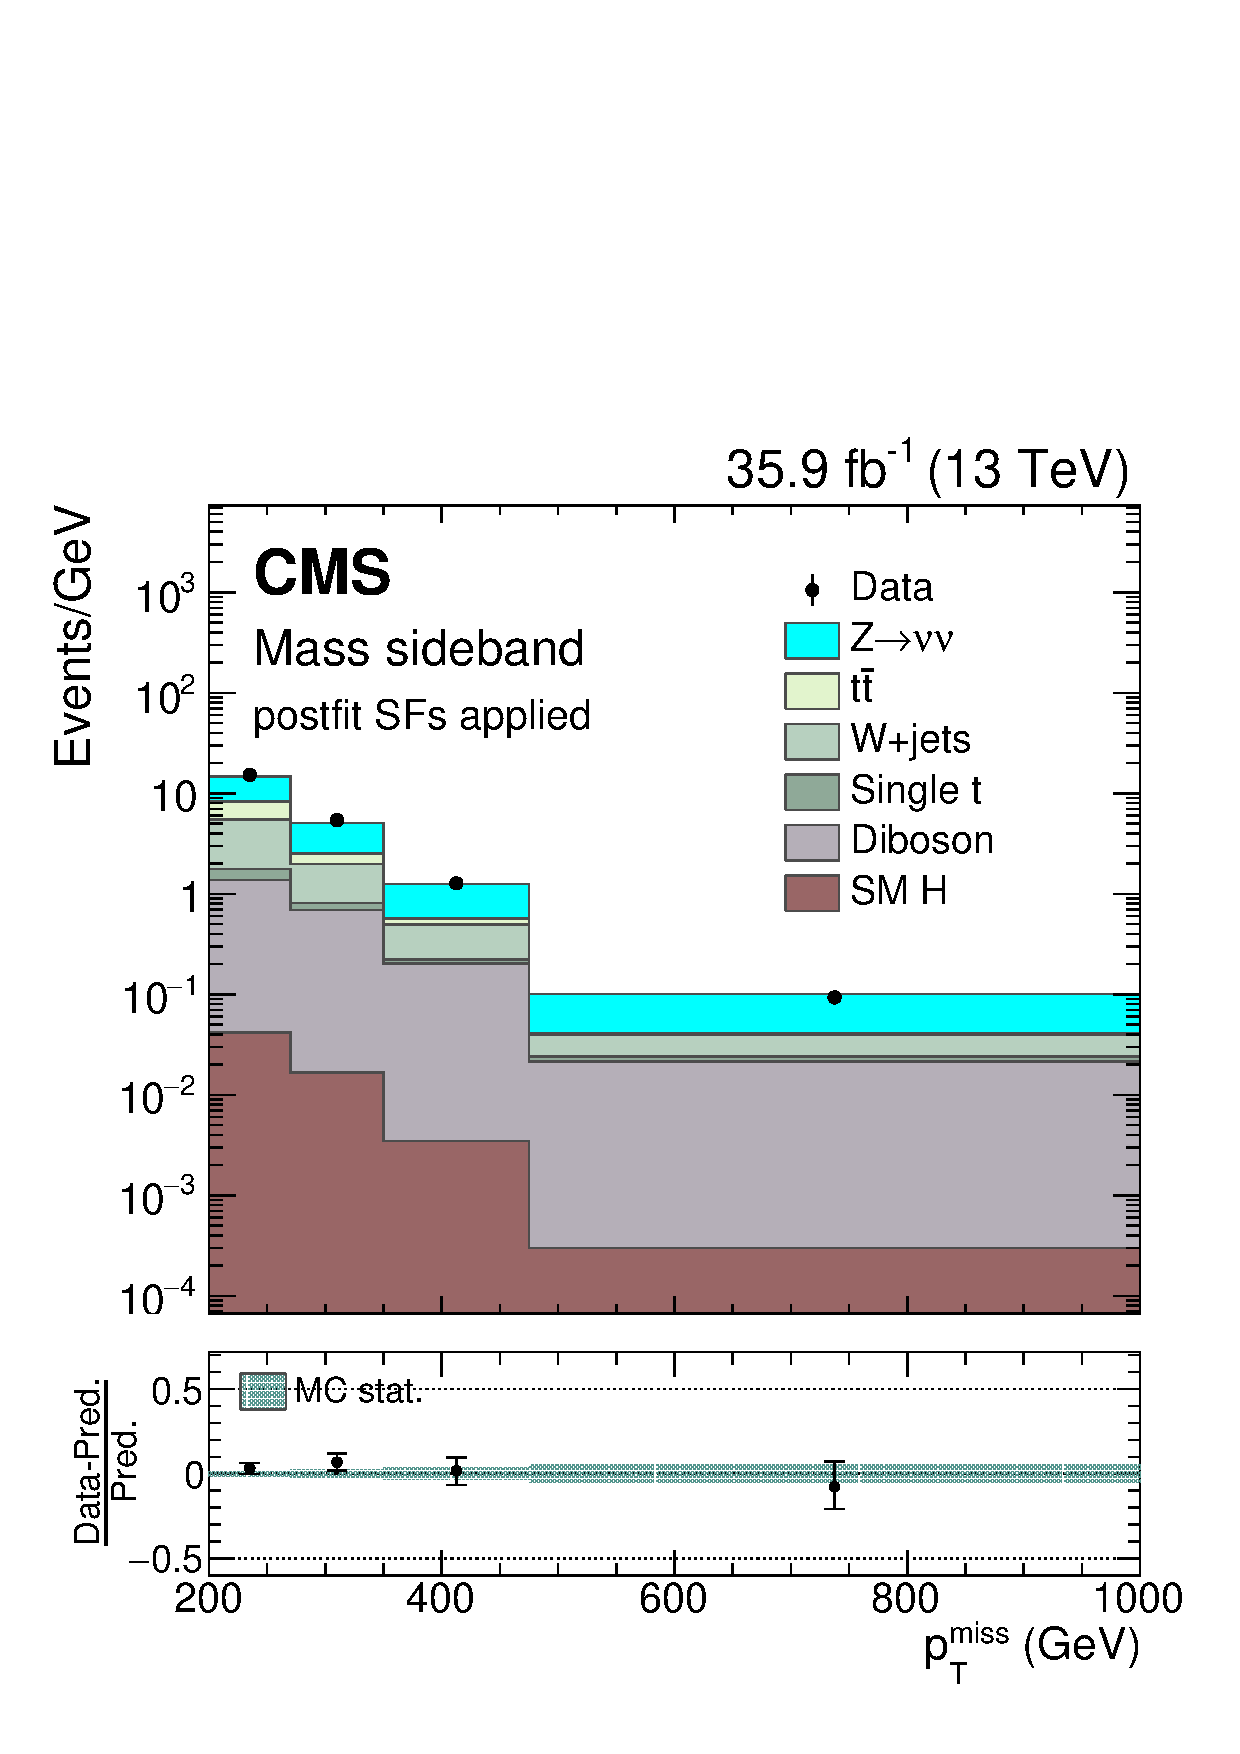
\includegraphics[width=0.4\textwidth]{figures/dataMC/cr_znunu_MET2_postfit.pdf}} \\
\caption{Left: prefit predictions in the mass sideband of the signal region. Right: postfit SFs for V+jets and \ttbar~processes obtained in the limit fit are applied to events in the sideband. A good agreement is observed, serving as additional cross check of the obtained fit results.}
\label{Fig_sideband}
\end{figure}

\subsection{Limits on model parameters}\label{subsec:limits}

Figure~\ref{fig:limits} shows the expected and observed exclusions as a function of $m_{Z'}$ and $m_{A^0}$ for the Z'-2HDM model and as a function of $m_{Z'}$ and $m_{\chi}$ for the Baryonic Z' model. Other assumptions are on $tan\beta = 1.0$, $g_{Z'} = 0.8$, and $m_{\chi} = 100$ GeV for the Z'-2HDM, while for the Baryonic Z' model couplings are assumed to be $g_{q} = 0.25, g_{\chi}=1$. For the Z'-2HDM model, we exclude a Z' mass of 2.3\TeV with an expected exclusion of 2.55\TeV for a mass $m_{A^0}=300\GeV$. The lower exclusion boundary is given by $m_{Z'}=600\GeV$. The largest $A^0$ mass we can exclude is 700\GeV for a corresponding Z' mass of 1.75\TeV, with an expected exclusion of $M_{A^0}=800\GeV$. These are the most stringent limits put on this model to this date. For the Z'-Baryonic model we can exclude masses below $m_{Z'}=1.45\TeV$. The expected exclusion is 1.75\TeV. This is the first time that limits on this model have been set in the mono-H(bb) channel. 
%The interpolation is done with a relatively rough grid, which will be improved.

\begin{figure}[htbp]
   \centering
   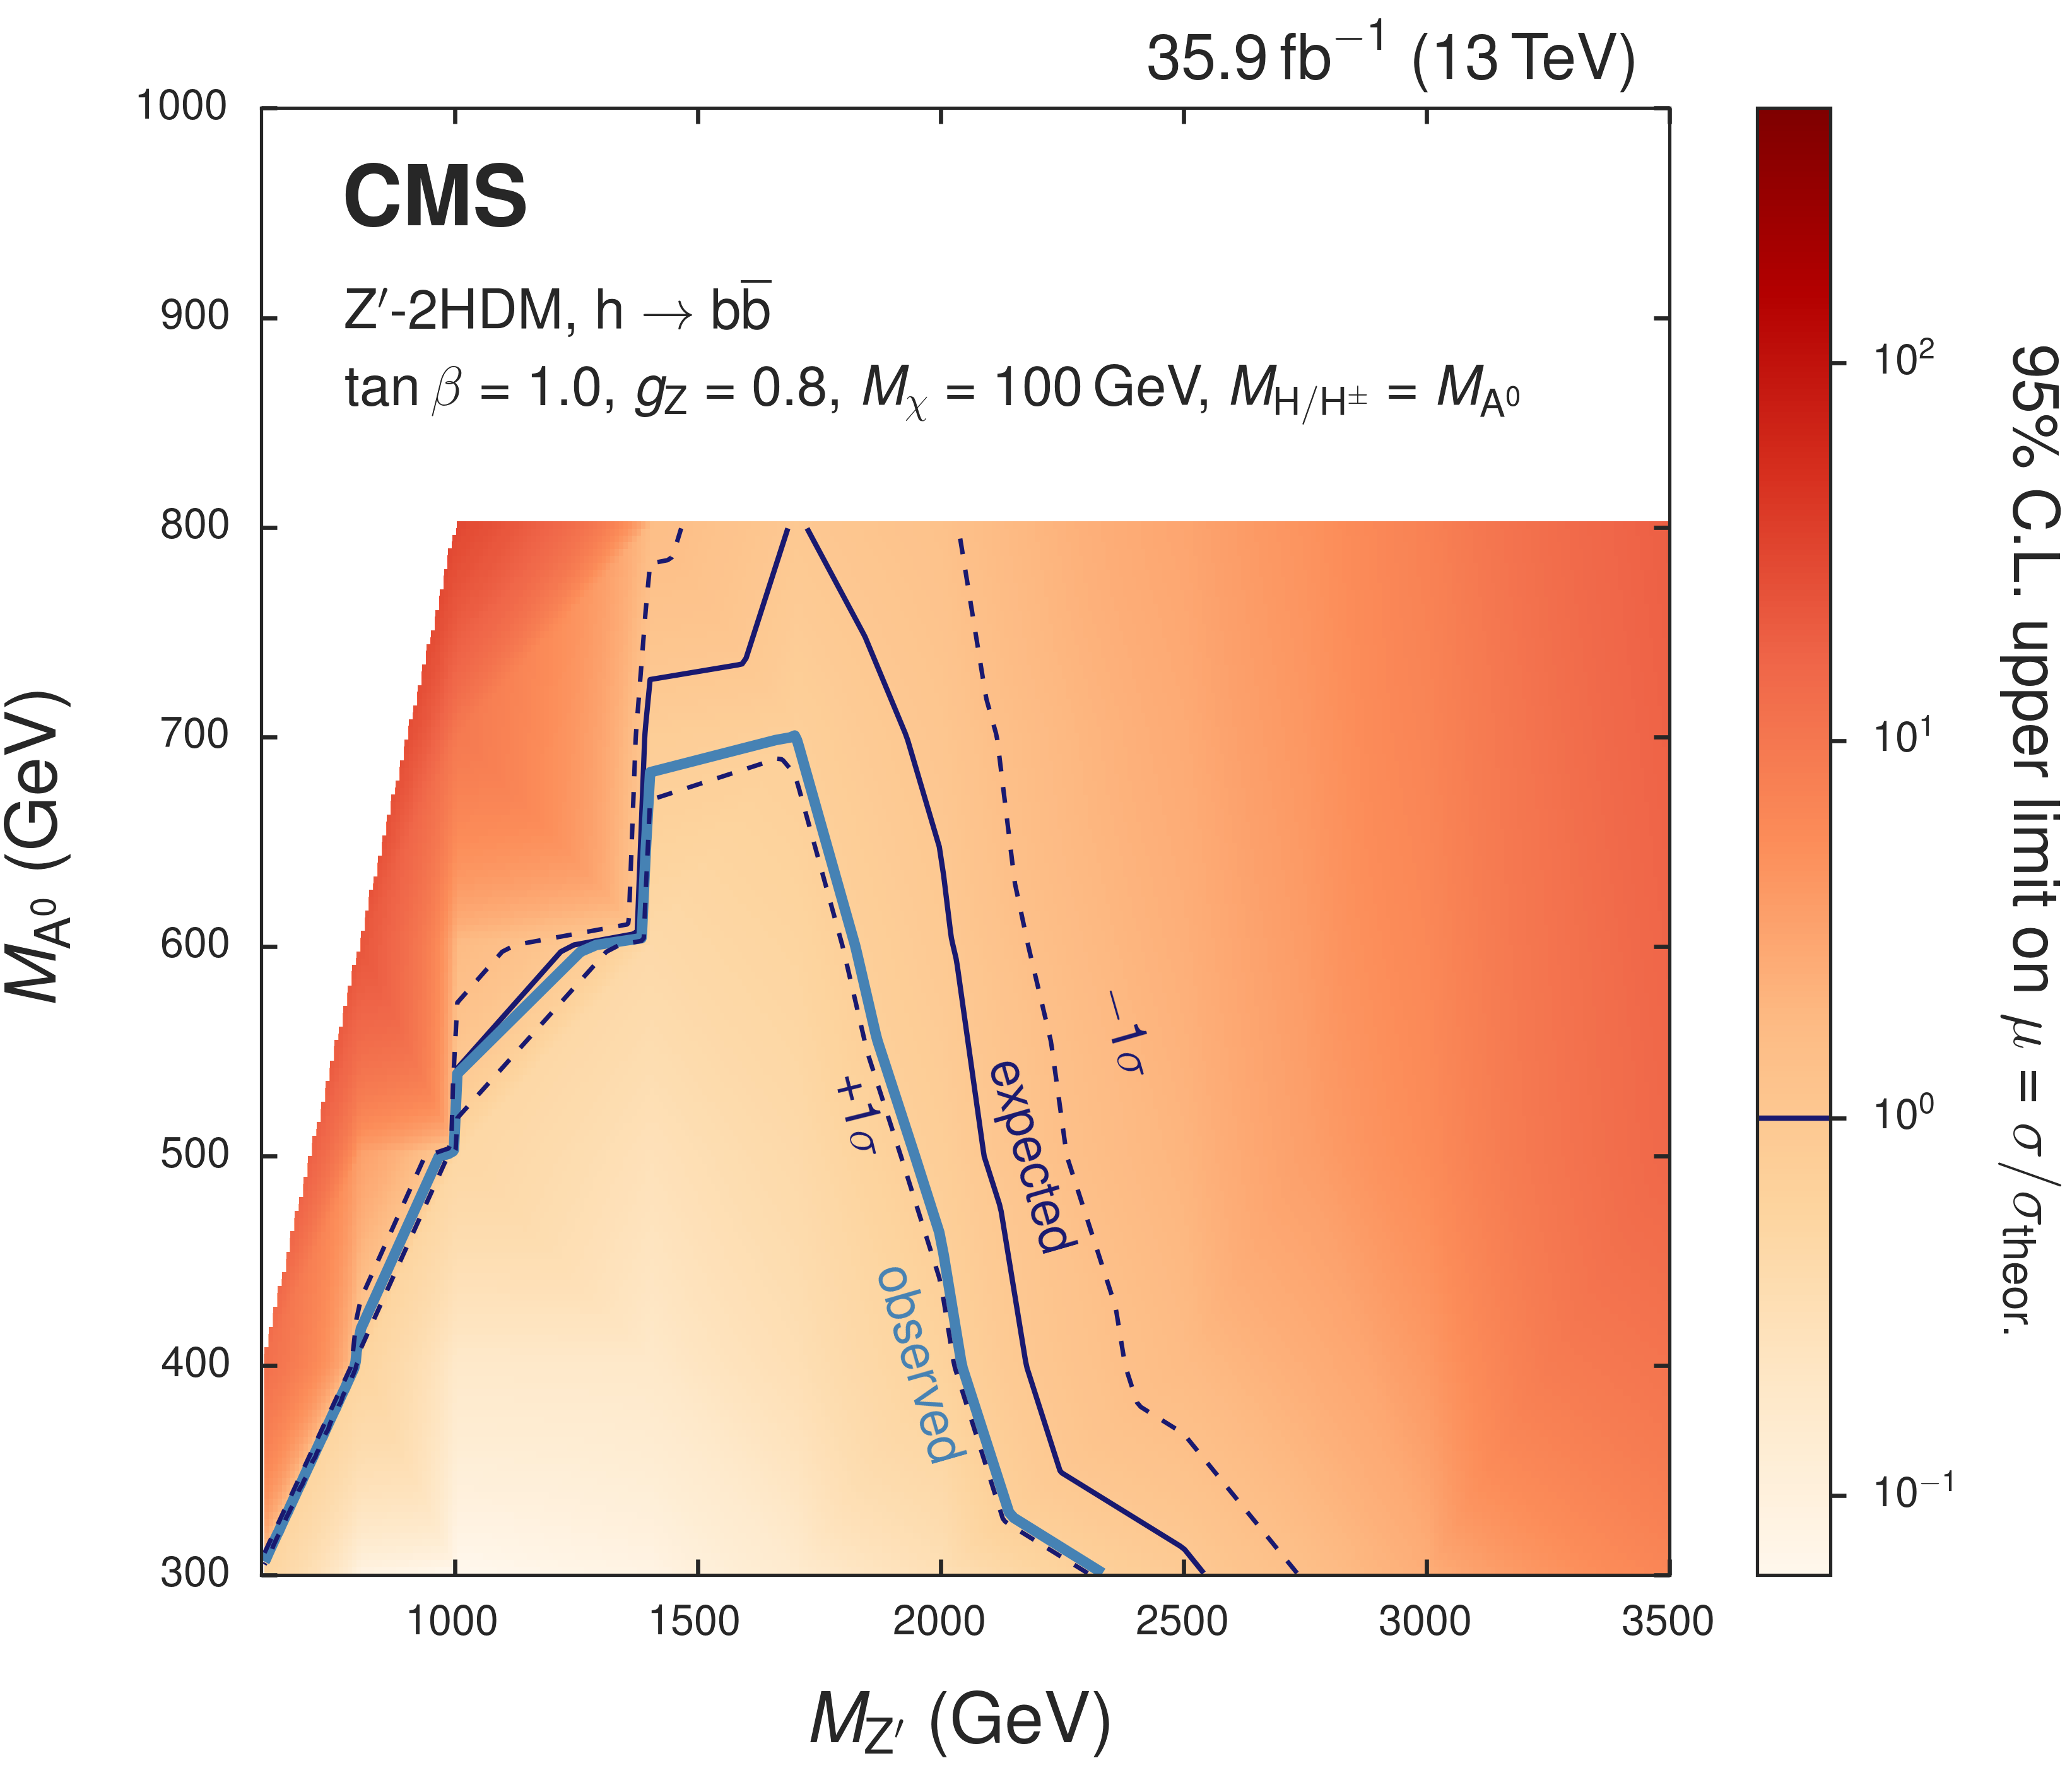
\includegraphics[width=0.475\textwidth]{figures/limits/limits_2hdm2d.png}
   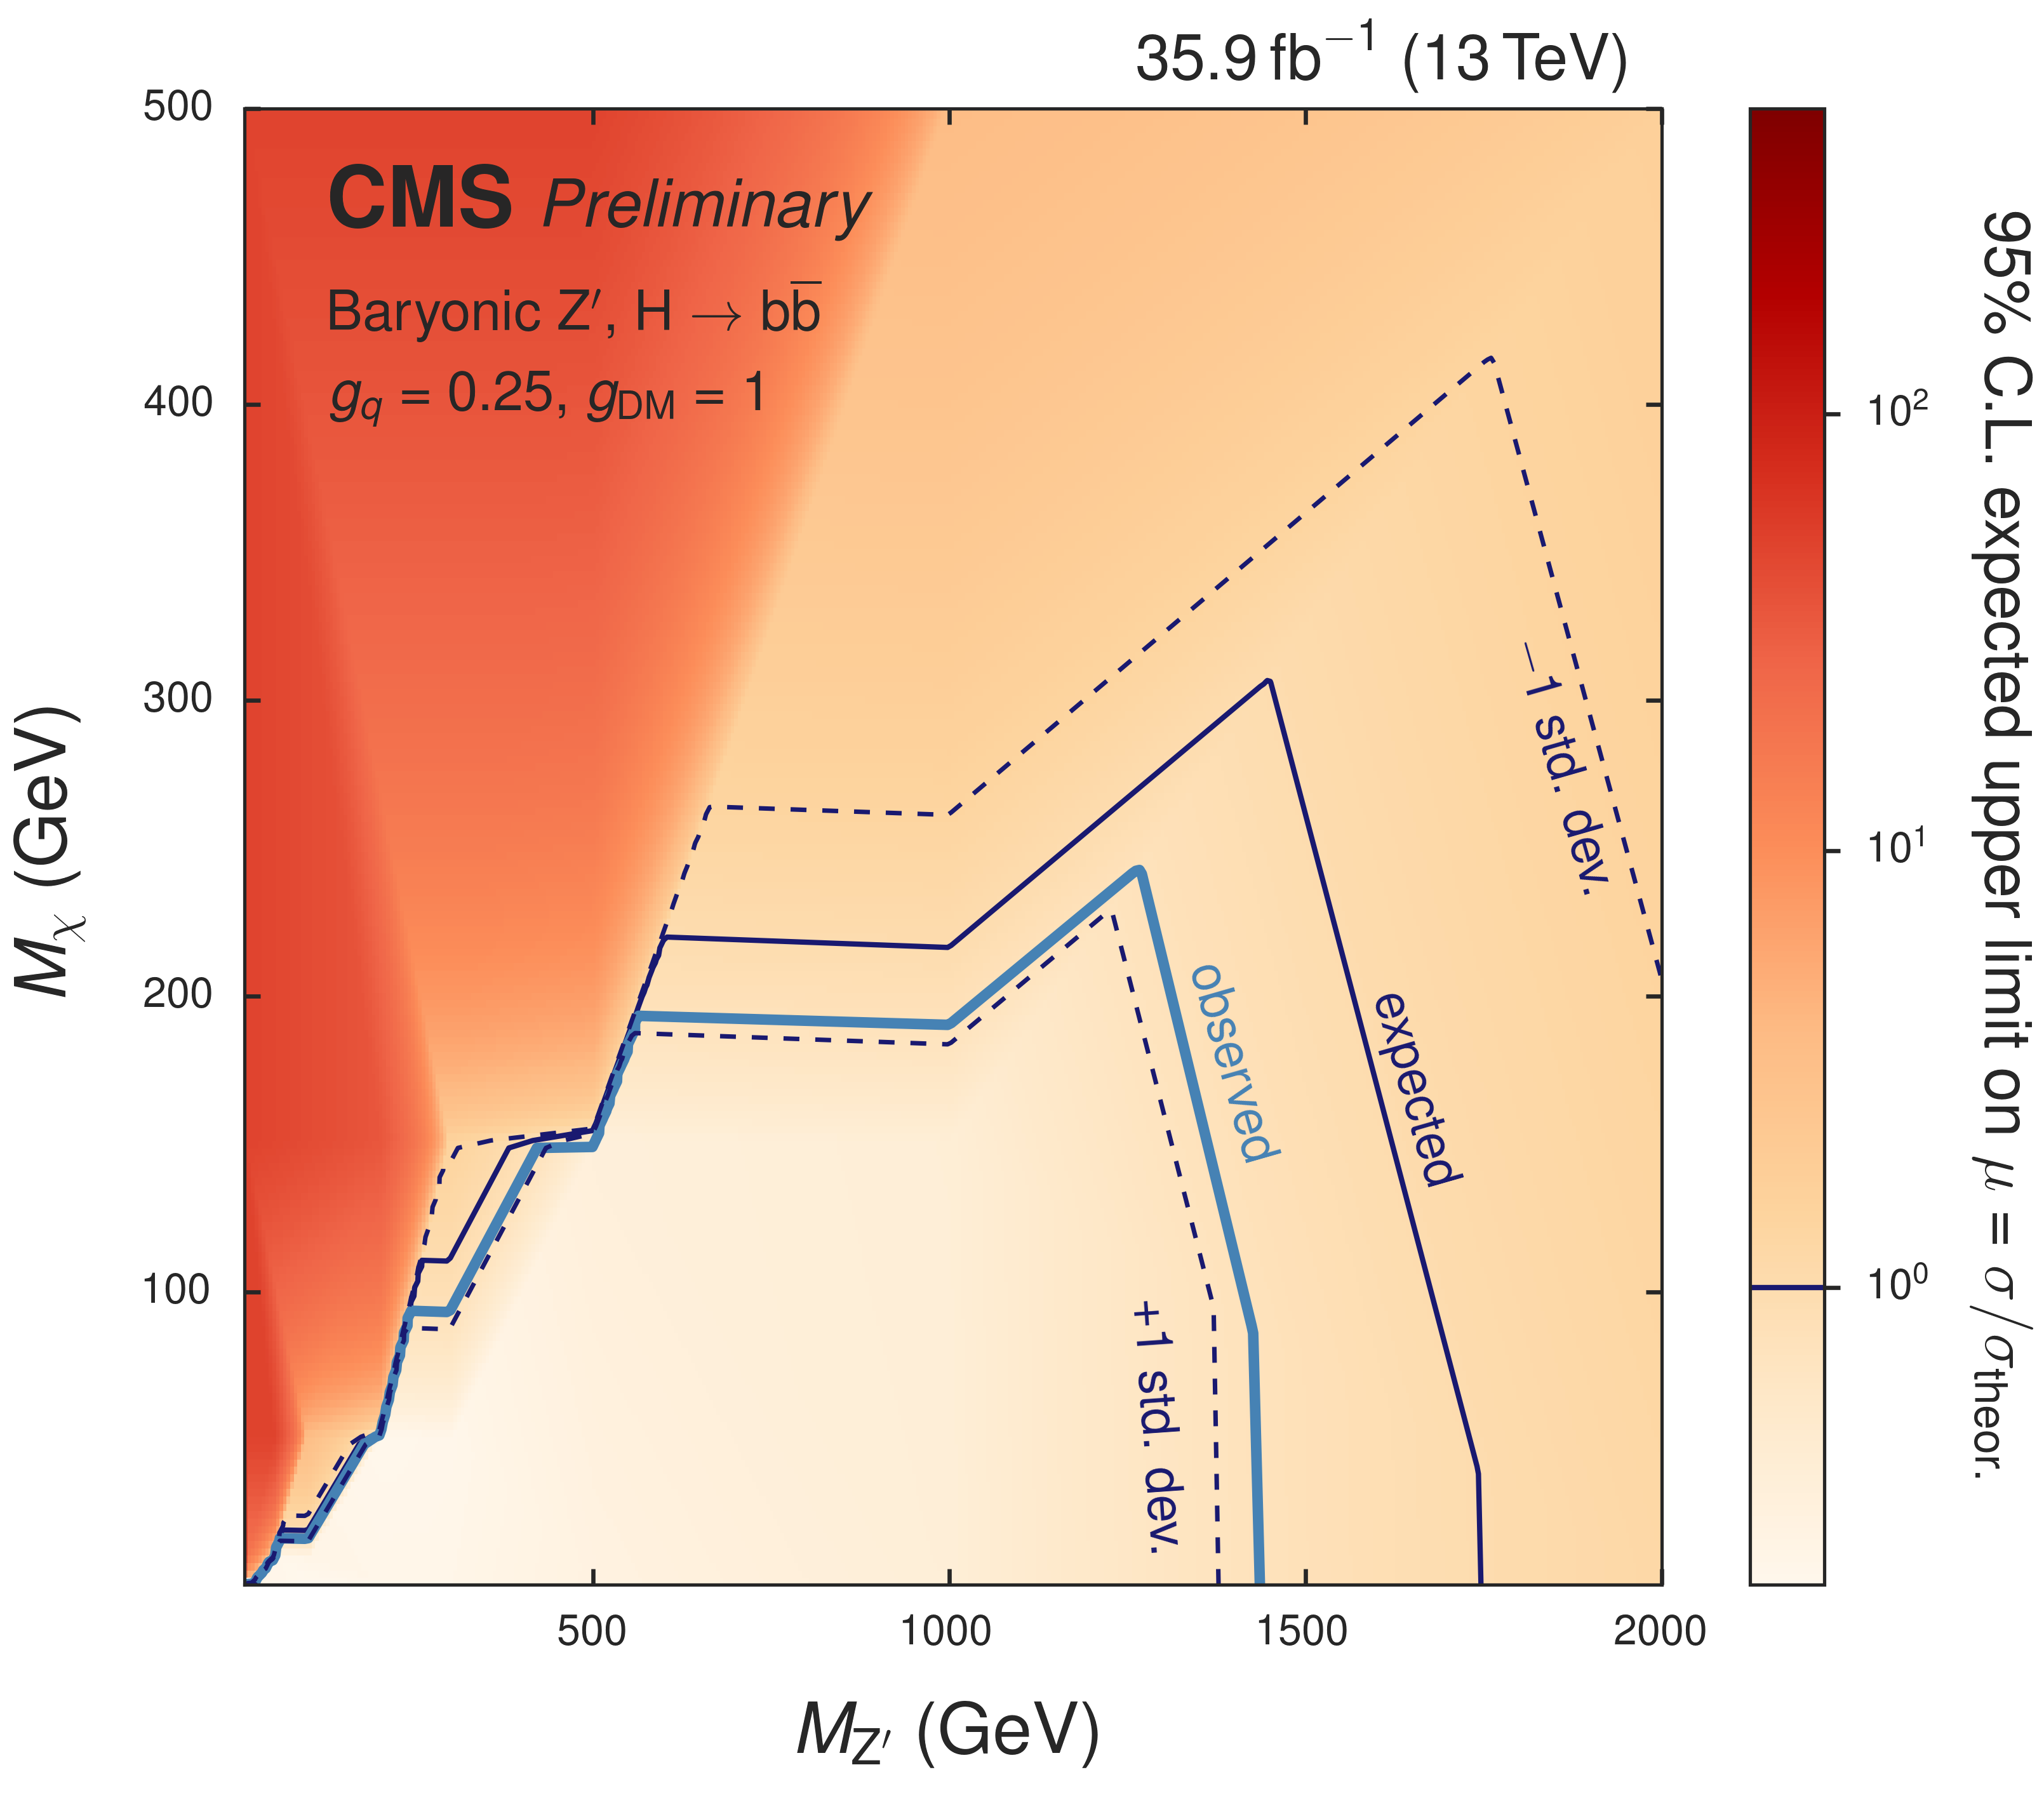
\includegraphics[width=0.475\textwidth]{figures/limits/limits_barzp2d.png}\\
   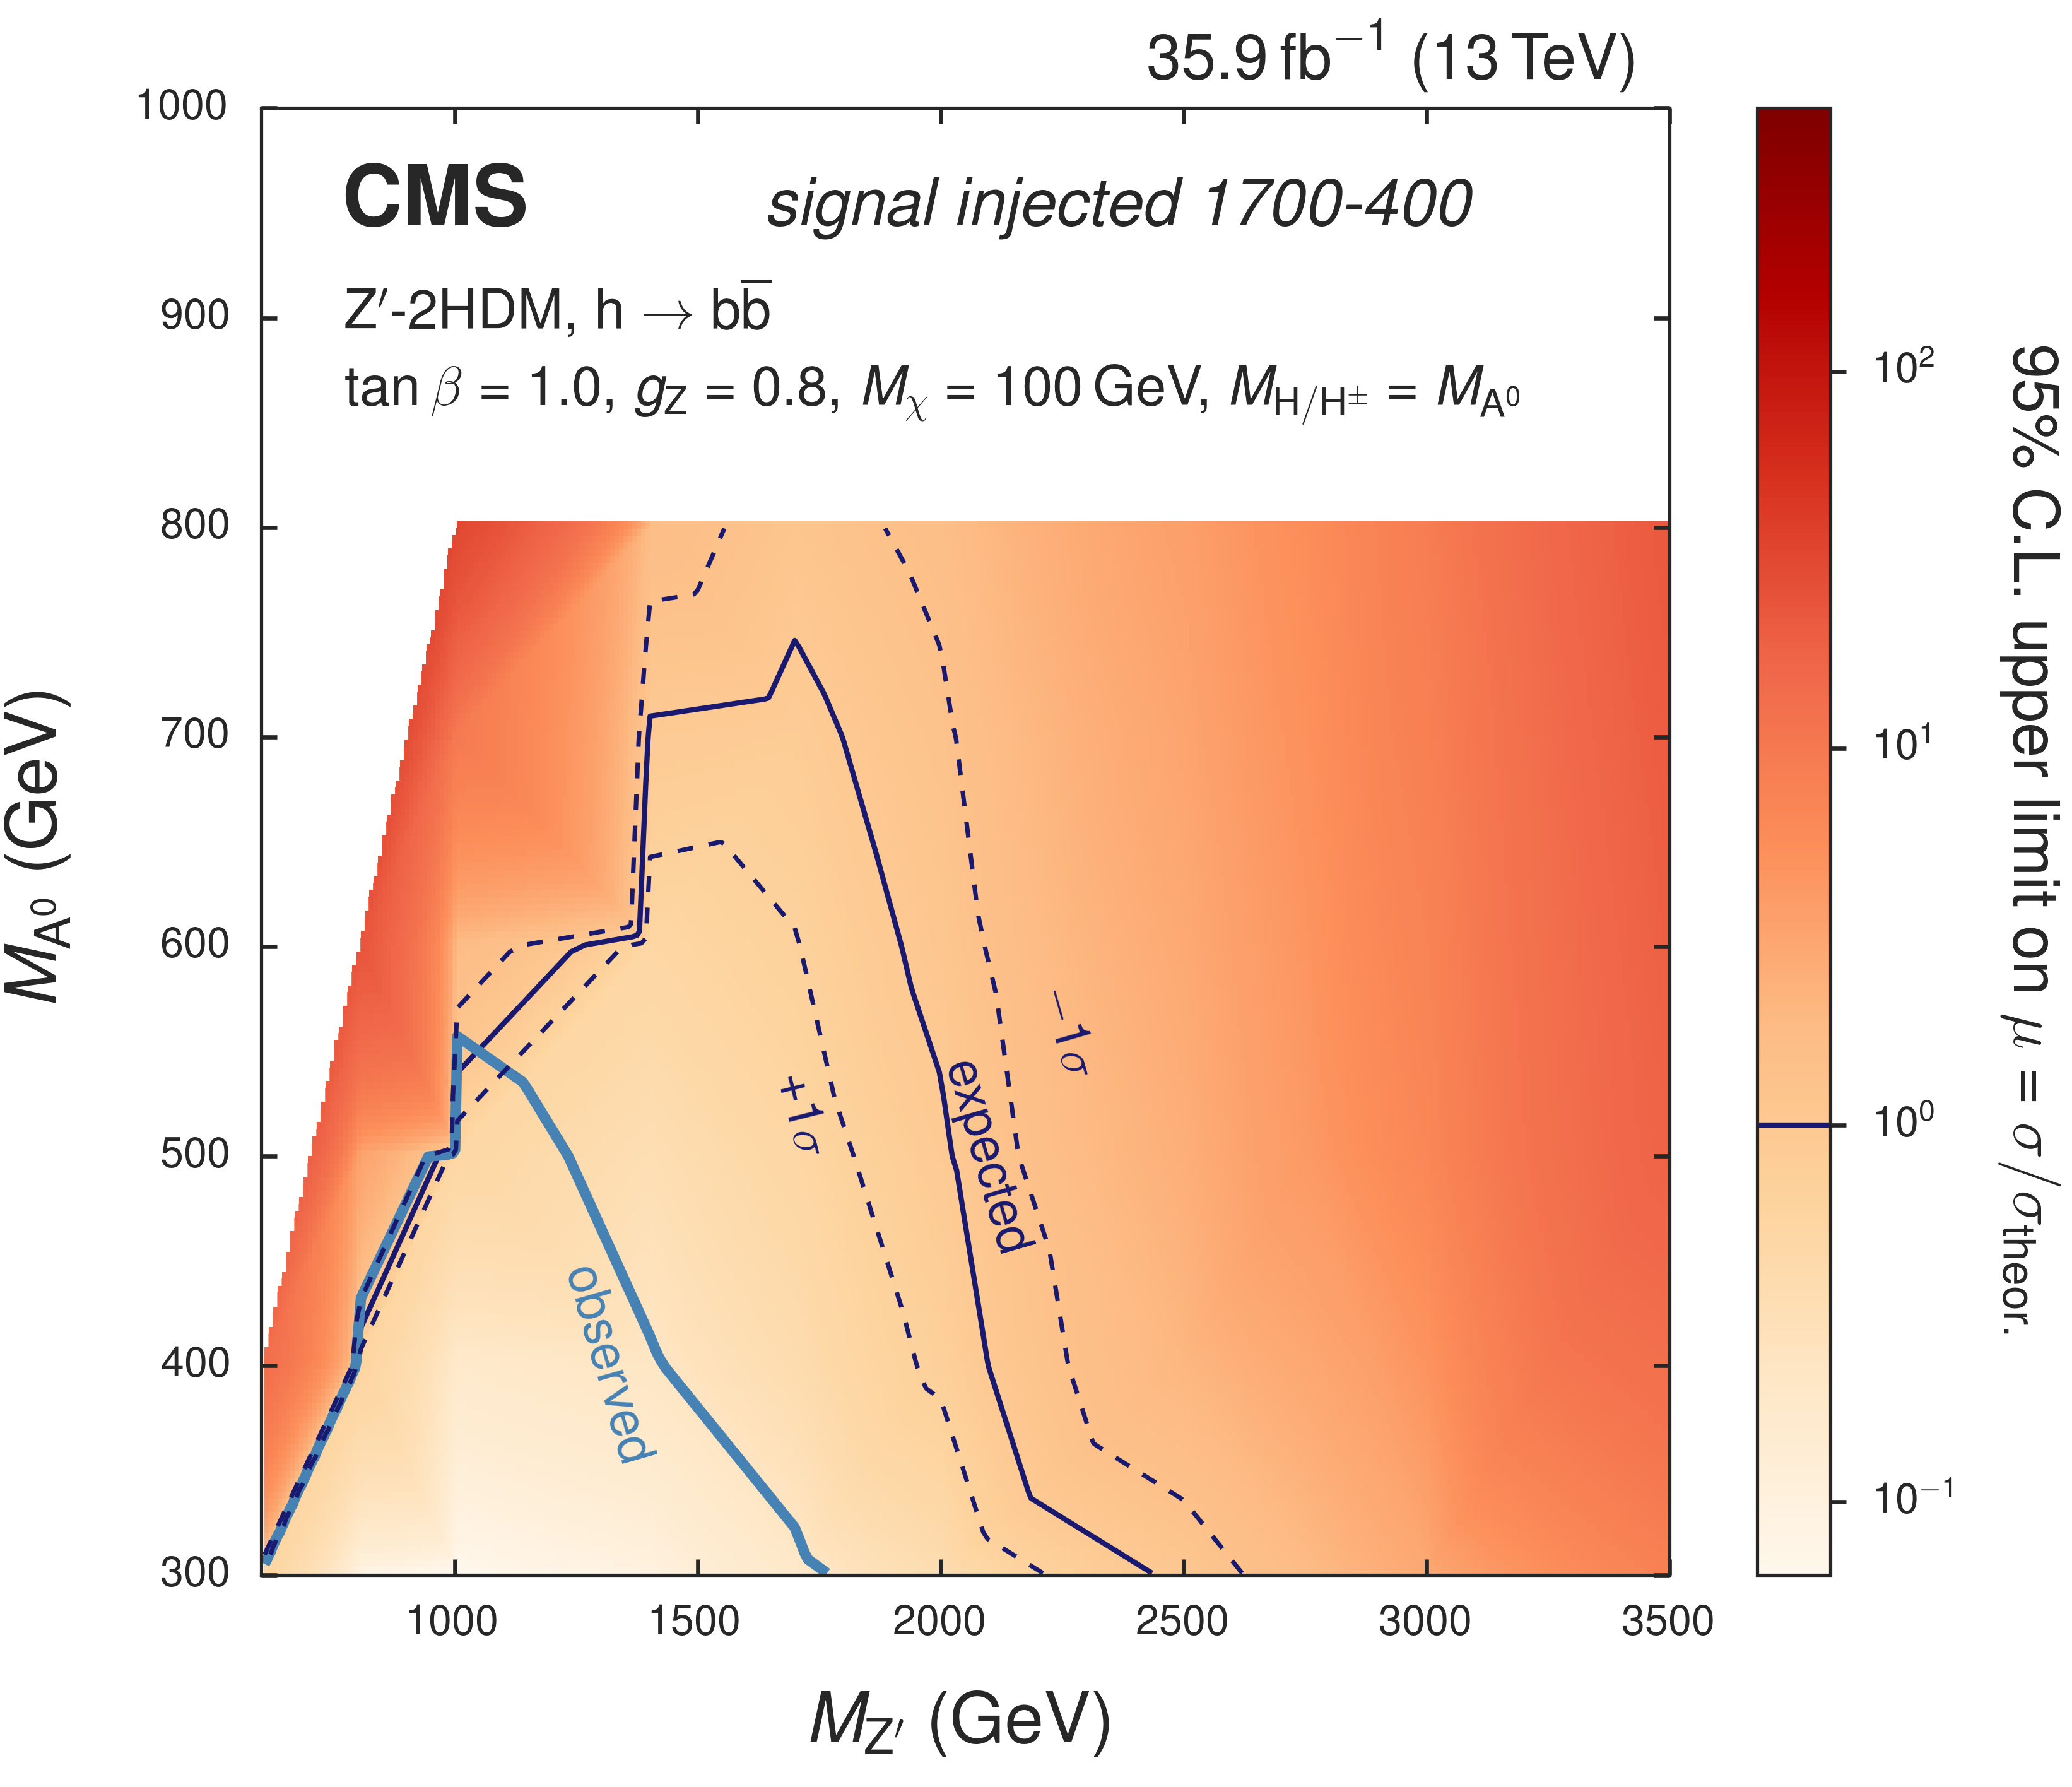
\includegraphics[width=0.475\textwidth]{figures/limits/limits_2hdm_siginj.png}
   \caption{Left: limits on the signal strength for the Z'-2HDM model. Right: limits on the signal strength modified for the Baryonic Z' model. Bottom: limits for the Z'-2HDM model if the data contain the signal scenario with $M_{Z'}=1.7\TeV$ and $M_{A^0}=400\GeV$.}
   \label{fig:limits}
\end{figure}

